\documentclass[%
  a4paper,              % DIN A4
  style=print,          % enables twoside, print colors, and BCOR=15mm
  bibliography=totoc,   % bibliography gets unnumbered entry
  nexus,                % corporate design font
  lnum,                 % use "Versalziffern" instead of "Mediaevalziffern"
  extramargin,          % override corporate design margin to give more space for one-column text
  %hyperrefdark,
%  smallchapters         % can optionally be enabled for smaller font size in chapter headings
]{tubsbook}

\usepackage[hidelinks]{hyperref}

\input{../lib/thesis_internal.tex}

\usepackage{tabularx}
\usepackage{pgfgantt} % Schedule
\usepackage[printonlyused]{acronym}
\usepackage{tikz}
\usepackage{tikz-uml}
\usepackage{booktabs}
\usepackage{pdflscape}
\usepackage{ifthen}
\usepackage{subfig}
\usepackage{enumitem}
\usetikzlibrary{trees,positioning,fit,arrows,decorations.pathreplacing}

\newcommand{\fitlab}{\emph{FIT IoT-LAB} }

\begin{document}
\frontmatter % roman page numbering

\maketitle
\cleardoublepage

% statement of originality
\thispagestyle{plain} % no header
\vspace*{7cm}
\ifgerman
	\centerline{\bfseries Eidesstattliche Erklärung}
	\vspace*{1em}
	\noindent
	Ich erkläre hiermit an Eides statt, dass ich die vorliegende
	Bachelorarbeit/Projektarbeit/Masterarbeit selbstständig verfasst sowie alle
	benutzten Quellen und Hilfsmittel vollständig angegeben habe und dass die Arbeit
	nicht bereits als Prüfungsarbeit vorgelegen hat.

	\par
	  \bigskip\noindent Braunschweig, den \thesisdate \par
\else
	\centerline{\bfseries Statement of Originality}
	\vspace*{1em}
	\noindent
	This thesis has been performed independently with the support of my supervisor/s.
	To the best of the author's knowledge, this thesis contains no material previously
	published or written by another person except where due reference is made in the text.

	\par
	  \bigskip\noindent Braunschweig, \thesisdate \par
\fi
  \vspace*{10mm}
  \hfill\hrulefill
\cleardoublepage

% abstract
\thispagestyle{plain} % no header
\centerline{\bfseries Abstract}
\vspace*{1em}
\noindent

The \ac{RPL} has evolved into one of the most commonly used routing protocols
for \acp{WSN}. It has already been evaluated under various criteria and for a
wide range of applications. Previous work has established that single or
multiple node restarts can transiently affect the rest of the network. The
implications of this effect motivated a consecutive work that implemented a
hardened version of \ac{RPL} based on the \emph{Contiki} operating system. The
implementation has then been evaluated both using the \emph{Cooja} network
simulator and a small test network. It has been concluded that the hardened
implementation significantly reduced the control message overhead for \ac{WSN}
in which single or multiple node resets occur.

This thesis builds upon these findings by evaluating the effect of transient
node failures using \fitlab, a large scale \ac{IoT} test network. For this
purpose software has been created which automates the execution of the
experiments and automatically collects and analyses the results.

The general effect of transient node failures on \ac{RPL} has been confirmed
using \fitlab. The hardened implementation manages to significantly reduce the
control message overhead of a recovering network, but increases the overhead if
no resets occur. Other criteria, such as the packet delivery ratio and the
network convergence time, are adversely affected by it.

\acresetall

%\vspace*{5em}
%
%\centerline{\bfseries Zusammenfassung}
%\vspace*{1em}
%\noindent
%Hier steht die deutsche Zusammenfassung, bei Arbeiten auf Deutsch steht die deutsche Zusammenfassung oben. If your thesis is in english, the german Zusammenfassung is optional.
\cleardoublepage

% include Aufgabenstellung pdf
% this is only needed if you did not write an expose/proposal
%\usepackage{pdfpages}
%\includepdf[pages=-]{aufgabenstellung/Aufgabenstellung}
%\cleardoublepage

\tableofcontents
\cleardoublepage

\listoffigures
\cleardoublepage

\listoftables
\cleardoublepage

\chapter*{Acronyms}

\begin{acronym}
  \acro{AM}{Averaging Mode}
  \acro{API}{Application programming interface}
  \acro{ASCII}{American Standard Code for Information Interchange}
  \acro{BFS}{Breadth First Search}
  \acro{CLI}{Command Line Interface}
  \acro{CN}{Control Node}
  \acro{CPU}{Central Processing Unit}
  \acro{Co-RPL}{Coronal RPL}
  \acro{CT}{Conversion Time}
  \acro{DAG}{Directed Acyclic Graph}
  \acro{DAO}{Destination Advertisement Object}
  \acro{DIO}{DODAG Information Object}
  \acro{DIS}{DODAG Information Solicitation}
  \acro{DODAG}{Destination Oriented Directed Acyclic Graph}
  \acro{ETX}{Estimated Transmission Count}
  \acro{GPIO}{General Purpose Input Output}
  \acro{GPS}{Global Positioning System}
  \acro{GW}{Gateway Node}
  \acro{HN}{Host Node}
  \acro{HTTP}{Hyper Text Transfer Protocol}
  \acro{I$^2$C}{Inter-Integrated Circuit}
  \acro{IBR}{Institut für Betriebsysteme und Rechnerverbund}
  \acro{ICMPv6}{Internet Control Message Protocol version 6}
  \acro{IDS}{Intrusion Detection System}
  \acro{IoT}{Internet of Things}
  \acro{IP}{Internet Protocol}
  \acro{IPv6}{Internet Protocol Version 6}
  \acro{ISM}{industrial, scientific and medical}
  \acro{JSON}{JavaScript Object Notation}
  \acro{JTAG}{Joint Test Action Group}
  \acro{LLN}{Low power Lossy Network}
  \acro{MAC}{Media Access Control}
  \acro{NUD}{Neighbor Unreachability Notification}
  \acro{OF}{Objective Function}
  \acro{OML}{O! Markup Language} % wtf
  \acro{ON}{Open Node}
  \acro{PCAP}{Packet Capture}
  \acro{PDR}{Packet Delivery Ratio}
  \acro{PM}{Periodic Measure}
  \acro{PRR}{Packet Reception Rate}
  \acro{RAM}{Random-access memory}
  \acro{REST}{Representational State Transfer}
  \acro{RPL}{Routing Protocol for low Power and Lossy Networks}
  \acro{RSSI}{Received Signal Strength Indication}
  \acro{RTC}{Real-Time Clock}
  \acro{RX}{Receive}
  \acro{SBC}{Single Board Computer}
  \acro{SD}{Secure Digital}
  \acro{SNMP}{Simple Network Management Protocol}
  \acro{SPI}{Serial Peripheral Interface bus}
  \acro{SQL}{Structured Query Language}
  \acro{SRAM}{Static Random-Access Memory}
  \acro{SSH}{Secure Shell}
  \acro{SoC}{System on a Chip}
  \acro{TCP}{Transmission Control Protocol}
  \acro{TUA}{Time Until Arrival}
  \acro{TX}{Transmit}
  \acro{UART}{Universal asynchronous receiver/transmitter}
  \acro{UDP}{User Datagram Protocol}
  \acro{UID}{Unique Identifier}
  \acro{USB}{Universal Serial Bus}
  \acro{VCC}{Voltage Common Collector}
  \acro{WSN}{Wireless Sensor Network}
\end{acronym}

\acused{API}
\acused{ASCII}
\acused{CPU}
\acused{GPIO}
\acused{GPS}
\acused{HTTP}
\acused{I$^2$C}
\acused{ICMPv6}
\acused{IP}
\acused{IPv6}
\acused{IoT}
\acused{JSON}
\acused{JTAG}
\acused{MAC}
\acused{RAM}
\acused{REST}
\acused{RSSI}
\acused{RTC}
\acused{RX}
\acused{SBC}
\acused{SD}
\acused{SNMP}
\acused{SPI}
\acused{SQL}
\acused{SRAM}
\acused{SSH}

\cleardoublepage

\mainmatter % arabic numbering

\chapter{Introduction}

In recent years, \acp{WSN} have been widely adopted as a means for applications
such as industrial monitoring \cite{ding2010sensing} \cite{rfc5673}, wild-life
tracking \cite{cassens2017automated} and public infrastructure \cite{rfc5867}.
One significant trend is the rise of networked embedded devices that contain
sensors and actors for performing dedicated tasks, which is often referred to as
the \acf{IoT}.

Many of these applications have in common that they need some means of
transporting commands to these embedded devices and in turn receive sensor data
from the devices. The way such a transport channel is achieved is often through
creating a wireless mesh network, since deployment is comparatively convenient
and cost efficient compared to wired networks. At the same time, such devices
will often be battery powered, since at the deployment side a connection to the
power grid might not be available with reasonable effort. In total, these
restrictions lead to different constraints on the software that creates the mesh
routing.

When nodes are supplied by a battery, the maintenance interval of the node
itself depends on how efficiently the node manages its limited amount of energy.
In extreme cases (e.g. where the sink depletes its battery first) the total
lifetime of the network may even depend on the minimum lifetime of any node in
the network. For routing in \ac{WSN} the amount of energy it takes to establish
a routing topology within the network of devices is largely due to the time the
radio is powered for transmitting messages, which is proportional to the number
and sizes of messages that need to be exchanged to create and maintain the
routing topology. The amount of energy used also depends on the efficiency of
the resulting routing topology when transmitting messages through the network.
There is often a trade-off between the energy consumption of a network and the
performance in terms of network latency and throughput. For this, different
metrics can be applied and have to be carefully selected based on the conditions
the network operates in.

A problem that often occurs, especially in harsh environmental conditions (e.g.
outdoor deployments, wildlife monitoring) or with faulty software, is from
single or repeated node restarts. When a node resets, it has to reconfigure its
routing information by exchanging message with surrounding nodes, which makes up
a great part of the energy costs associated with \ac{WSN}. Such restarts do not
only affect the specific resetting node, but also nodes that depend on the
resetting node inside the routing topology. Previous work has shown that this
behavior of transitively failing nodes can have a large impact on the energy
efficiency of \acp{WSN} using \ac{RPL} \cite{kulau2017energy},
\cite{mueller2017}.

The \ac{RPL} is a protocol for routing messages in wireless mesh networks
and has explicitly been designed for use with networks of nodes with low power
consumption and lossy wireless links, as is typical for many deployment
scenarios. It has become the de-facto standard routing protocol for wireless
sensor networks and, as such, its behavior in conditions where transient node
failures occur is of great interest to this work.

One aspect of the effectiveness of a mesh routing protocol is how it deals with
such transient node failures. It has to quickly detect these failures, decide
how to invalidate the routes using the failed node and create and announce
alternative routes in the network.

In subsequent work \cite{mueller2017}, a hardened implementation of \ac{RPL} for
the \emph{Contiki} operating system has been developed, that managed to reduce
the influence of node restarts, by restoring a previous state that has been
stored in the flash memory of the node. This hardened implementation has
previously been evaluated both using simulations and within a limited test
network.

The \fitlab is a shared \ac{IoT} test network that features over 2000 nodes and
provides an interface for the remote configuration and scheduling of
experiments. Measurement data can be obtained for a variety of variables including
\ac{RSSI}, \acp{PCAP}, serial interface output, and event logs for each node.
The goal of this work is to further verify the findings concerning the effect of
node restarts on the performance of \ac{RPL} and to evaluate the effectiveness
of the hardened implementation for reducing the energy impact of transient node
failures on a larger scale. In addition to the parameters needed for the
verification of previous work \cite{mueller2017}, some further variables have
been recorded (see \autoref{tab:params}) and evaluated that allow some
conclusion about the performance \ac{RPL}.

In \autoref{chap:relwork} an introduction to the mechanisms of \ac{RPL} is given
and other work discussing the protocol performance of \ac{RPL} is presented
including an analysis of the effect of transient node failures in \ac{WSN}. From
the literature, different attempts for hardening \ac{RPL} against various forms
of attacks on the protocol and other extensions that aim to add security and
better performance are presented.

The topology of test network and the hardware used for the sensor nodes is
descibed in \autoref{chap:hardware}, while in \autoref{chap:setup} the different
software components are further described including how the data for the
individual variables is recorded, aggregated and analyzed.

In \autoref{chap:evaluation} a description of the different configurations the
experiments were run in, how parameters were controlled is given for and the
analysis of the network topology, network performance and energy consumption is
are presented.
\chapter{Related Work} % English: Related Work
\label{chap:relwork}

Much work has been done evaluating \ac{RPL} and its repair process.
In the following, a brief introduction to \ac{RPL} will be given, then previous research concerning the general performance of the protocol will be presented.
After this, an overview of the sources of unreliability in \ac{WSN} follows and resetting nodes as a factor for network disruption are considered in more detail, before work is presented discussing the effects of the resulting transient node failures in more detail.
From the literature, extensions to \ac{RPL}, that may help to improve protocol reliability and network lifetime, will be presented, including optimizing the \ac{OF} for network lifetime, improving the formation of network paths, implementing fairer broadcast suppression, using intrusion detection systems, adding trust and authenticity and storing routing information persistently.

\section{Introduction to RPL}

\ac{RPL} as defined in \cite{rfc6550} is a routing protocol for \acp{LLN} that provides energy efficient networking for resource-constrained devices in networks where interconnects are expected to be bidirectional, but may have low data rates, high error rates and be unstable.
In \ac{RPL}, nodes self-organize to form a \ac{DODAG}, where the node with the lowest rank is the destination of and the root of the \ac{DAG}.
Such a \ac{DODAG} is displayed in \autoref{fig:dodag}.

The bootstrapping process defines how nodes may join the network by selecting a parent and how to globally or locally repair the network when necessary.
Each node emits \ac{DIO} messages targeted at all nodes in transmission range.
These messages advertise the presence of a node, its affiliation with an existing \ac{DODAG}, the current routing costs and related metrics.

A joining node may receive these messages and select a parent in the \ac{DODAG}
based on the received rank and routing costs, but must not select a node with a rank lesser than its current.
The separation of the route metric from the forwarding process is an important characteristic of \ac{RPL} as the function that is used to calculate the route metric, the \ac{OF}, can be exchanged to form \acp{DODAG} based on different characteristics.

\begin{figure}[h]
  \centering
  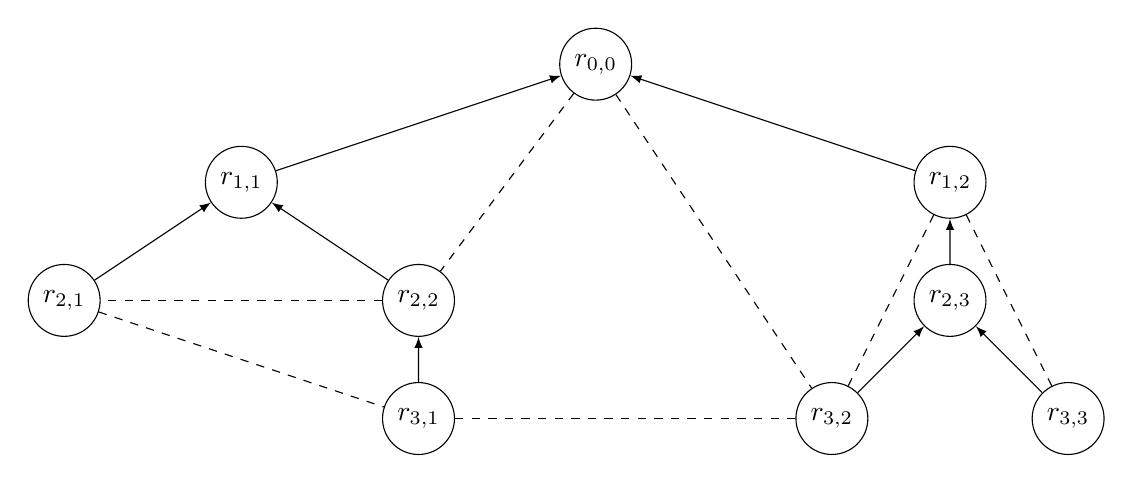
\begin{tikzpicture}[edge from parent/.style={draw,latex-},
      every node/.style={circle,draw},level/.style={sibling distance=90mm/#1}]
    \node (s) {$r_{0,0}$}
    child { node {$r_{1,1}$}
      child { node (d) {$r_{2,1}$}}
      child { node (a) {$r_{2,2}$}
        child { node (f) {$r_{3,1}$} }
      }
    }
    child { node (c) {$r_{1,2}$}
      child { node {$r_{2,3}$}
        child { node (b) {$r_{3,2}$} }
        child { node (e) {$r_{3,3}$} }
      }
    };
    \path (s) edge[dashed] (a);
    \path (s) edge[dashed] (b);
    \path (c) edge[dashed] (b);
    \path (a) edge[dashed] (d);
    \path (c) edge[dashed] (e);
    \path (d) edge[dashed] (f);
    \path (f) edge[dashed] (b);
  \end{tikzpicture}
  \caption{\acf{DODAG}}
  \label{fig:dodag}
\end{figure}

\section{Protocol Performance}

One of the main goals of this work is to evaluate the performance of \ac{RPL} when dealing with transient node failures.
Much research has already been done concerning the general performance of \ac{RPL}.

An extensive survey of energy efficient routing protocols is presented in \ac{WSN} \cite{pantazis2013energy}.
They classify protocols into four main categories, what their forwarding descisions are based on: network structure, communication mode, topology based and reliable routing.
\ac{RPL} is listed as as a reliable routing protocol and further subcategorized as a multipath-based protocol.
As an advantage they list low energy consumption, as a drawback that it only supports unicast traffic.
The scalability is rated as good, as is mobility and robustness.

The effectiveness and performance of \ac{RPL} has been evaluated in many publications \cite{rfc6687,accettura2011performance,korte2012study,ali2012performance,banh2015performance}.
In \cite{rfc6687}, the authors studied \ac{RPL} both in test networks of varying sizes and in simulations.
For the simulations, the link failure model and the network topology have been derived from measurements gathered from real-life deployments.
Simulations were performed using the \emph{OMNet++} \cite{varga2008overview} network simulator.
The authors measured path quality, routing table size, delay bounds, control overhead and connectivity loss.
The study does not directly consider network lifetime and energy consumption as a metric, but results where obtained pertaining to the scalability and performance under realistic scenarios.
It has been found, that \ac{RPL} scales well to very large topologies, provides near optimum path quality, neglible control overhead, and meets desired delay and convergency requirements for the given scenarios.
They also find, that with \ac{RPL} it is possible to tradeoff routing stability for less control overhead and thereby increase network lifetime.

A detailed study of \ac{RPL}, with a range of different parameter settings, as well as a comparison of the OF0 \cite{rfc6552}, which tries optimize for connectivity, and the \ac{ETX}-based \acp{OF} can be found in \cite{ali2012performance}.
Observations where made using the \emph{Cooja} \cite{osterlind2006cross} network simulator for \emph{Contiki}, energy usage has been measured using \emph{Powertrace} \cite{dunkels2011powertrace}.
Results hint to the importance of the settings for the Trickle timer for resource utilisation and the measured parameters.
The \emph{ContikiMac} \cite{dunkels2011contikimac} duty cycling is also found to be beneficiary to energy efficiency.
The findings also include results concerning network latency, delivery ratio, convergence time, control overhead and the energy consumption, using OF0 and \ac{ETX} respectively.
The tendency of node failures to be frequent and often transient is remarked at one point, but the effects were studied explicitly.

In \cite{korte2012study} the \ac{RPL} repair process is studied in more detail.
They evalutate a limited test network using the \emph{Contiki} \ac{RPL} implementation and studied the effect of node failures on the formation of the \ac{DODAG} before it undergoes local or global repair.
Here, the duration of the repair process and its individual steps are recorded and evaluated, as well as the results.
They were also able to confirm that the repaired \ac{DODAG} still matches the optimal \ac{DODAG} created by the \ac{OF}.
Although \cite{korte2012study} did not consider the additional energy usage from node failure, they find that most of the time it takes to recover from failure is spent on detecting a failed node, which may be useful when optimising the energy efficiency of the recovery process.
They also hint at the ability of \ac{RPL} to make use of an \ac{OF} that uses the remaing energy of a node as a metric.
This may help to balance energy consumption inside the network and thereby increase overall network lifetime.

While multiple other studies find that simulations of \ac{RPL} and experimental
results are largely consistent, Korte et al. \cite{korte2012study} measured a noticeable difference when comparing experimental results to simulations made in the network simulator \emph{NS2}\footnote{\url{https://www.isi.edu/nsnam/ns/}}.
They also remark that, for some situations, the time at which certain protocol messages must be send is underspecified in \ac{RPL}.
Depending on implementation details, these may lead to the creation of loops, which make it necessary to initiate a global repair of the \ac{DODAG}.
Additionally, the \ac{NUD} employed in \ac{RPL} may not be indicative for a loss of connectivity if higher layer protocols that function across longer than one hop paths, like \ac{TCP}, are used as an indication of connectivity.

When it comes to the effects of failing nodes, most research focuses on the performance of the local and global repair processes, but either it does not consider the possibility of transient node failure, or neglects the effects on the network lifetime from the resulting increased energy usage.

\section{Sources of Unreliability in WSN}

When evaluating networks with failing nodes, it is important to differentiate
the underlying cause for the failure, since failures from different causes may
exhibit different behavior concerning frequency, duration, and intensity of the
fault. As an example, while an error in programming for an edge-case may result
in only a single node restart, failures from overheating may be result in many
consecutive restarts. \cite{boano2013hot,boano2010impact}

The sources of unreliability in \ac{WSN} can be classified into those where an active attacker is involved and those where unreliable behavior is caused by passive environmental conditions.

%In energy constrained devices such as wireless sensor nodes, duty cycling is an important mechanism for conserving energy.
%One example of this is \emph{ContikiMAC} \cite{dunkels2011contikimac}, where the radio is only enabled for certain intervals of time.
When undervolting a sensor node, components of the nodes are run outside of their specified voltage range.
While this presents an interesting opportunity to increase the lifetime of \acp{WSN}, it may also increase the error rate of components and therefore may cause unpredictable behavior or even temporary node failure \cite{kulau2015undervolting}.
An implementation of undervolting for \ac{WSN} has been done by \cite{kulau2016idealvolting}.
They use supervised learning to adapt the voltage levels for individual nodes based on clock speed, temperature variations and differences in the manufacturing process.
This made it possible to prolong the lifetime of the network by more than 40\%.

Besides undervolting, there are many other factors in \ac{WSN} that may cause temporary node failure, such as temperature variations \cite{boano2010impact,boano2013hot,reynolds1974thermally}, programming errors and faulty components.

An overview of common active attacks against \acp{WSN} is presented by Karlof et
al.\cite{karlof2003secure}.
Surveyed modes of attack include: spoofed, altered, or replayed routing information, selective forwarding, sinkhole attacks, Sybil attacks, wormholes, HELLO flood attacks and acknowledgement spoofing.
As an ad-hoc, hierarchical routing protocol, \ac{RPL} is generally vulnerable against all of the described attacks.

\section{Effects of Transient Node Failures}

One attack not explicitly mentioned in \cite{karlof2003secure} is based on repeatedly restarting nodes as a possible attack vector.

Depending on the topology of the network, a single restarting node may cause transient node failures in other parts of the network and significantly increase the overall energy consumption of the network \cite{kulau2017energy}.
This may also be exploited by an active attacker.
Attacker controlled nodes integrate with the network, possibly using wormholing, in a way that as many paths as possible include the nodes as their parents.
The nodes then fail for a short time and subsequently restart.
By coordinating the timing and spacing of the restarts, an attacker repeatedly forces the network to repair itself.
As this behavior may also be triggered by malfunctioning nodes, such an behavior
may also be triggered accidentally.

In \cite{kulau2017energy}, the energy impact of single node restarts when using \ac{RPL} is studied in detail.
Experiments were done using the \emph{Cooja} network simulator and then compared to a reference simulation without resetting nodes.
Both the effect of single node restarts and multiple node restarts were investigated on a binary tree topology and for a meshed network, where each node can have more than one parent.
They discovered that a single node restart leads to an increased energy consumption of up to 20\% for the restarting node and its direct neighbors.
To remedy the effect of passive node failure, they suggest optimising \ac{RPL} parameters and keeping persistent information across node restarts, while, in case of an active attacker an \ac{IDS} would be more applicable.

\section{Extensions to RPL}

While \ac{RPL} is comparatively easy to implement, it has some weaknesses when it comes to mobility, energy consumption and packet delivery rates.
Some research that was done to extend and improve the protocol is presented here.

\subsection{Objective Functions}

An \ac{OF} is the function by which \ac{RPL} selects a parent in the \ac{DODAG} based on a metric like end-to-end delay, energy usage or delivery probability.
Since, in \ac{RPL}, the choice of \ac{OF} is independent of the forwarding mechanism, it is possible to substitute an \ac{OF} that produces a \ac{DODAG} that will be less effected by certain types of failure conditions.
A network can even have multiple \acp{DODAG}, that each can be optimized for different use cases.
Kamgueu et al. Kamgueu et al. \cite{kamgueu2013energy} implemented an \ac{OF} that uses the remaining energy of a candidate parent as a metric.
This way it is possible to create a \ac{DODAG} that distributes energy usage within the network more evenly and therefore increases network lifetime.
As opposed to computing the total energy level of a path, the costs for a path is the minimum energy level of any node in the path.
The \ac{OF} is evaluated using the \emph{Cooja} simulator for a network of 20 nodes.
They where able to increase network lifetime by around 14\% compared to a network using the \ac{ETX}-based \ac{OF}.
At the same time, the energy-based \ac{OF} achieved around 3\% worse delivery ratio compared to the \ac{ETX}-based \ac{OF}.
They note that future work would be needed to combine \ac{ETX} and energy-based \ac{OF}, to obtain both long network lifetime and a stable network.

\subsection{Coronal RPL}

In \cite{gaddour2014co} \ac{Co-RPL} is proposed as an an extension to \ac{RPL} and evaluated.
Co-\ac{RPL} makes use of the Corona mechanism \cite{olariu2006design} to help in the selection of a parent router and includes a procedure for reducing packet loss in case of a failing parent node.
It has been found that, in specific scenarios, \ac{Co-RPL} reduces end-to-end delay by up to 2.5 seconds, packet loss by up to 45\% and energy consumption by up to 50\%.

\subsection{Trickle Timer}

The time and therefore energy needed for a failed node to re-join the network is also influenced by the behavior of its \emph{Trickle} timer \cite{levis2004trickle}.
For \ac{RPL}, such a timer, based on the number of messages received during a sensing interval, regulates if the sender may send messages after the sensing interval.
Since the behavior of the \emph{Trickle} timer for networks of more than one node is inherently non-deterministic, it is possible that the share of sending time each node gets may be unfair \cite{vallati2013trickle}.
This in turn can result in less than optimal route selections when sensing for possible parents during the bootstrapping process.
\emph{Trickle-F} \cite{vallati2013trickle} is an attempt at adding fair broadcast suppression to the \emph{Trickle} algorithm.
Evaluations have shown its validity and that it was possible to obtain more efficient routes with same power consumption as the original algorithm.

\subsection{Intrusion Detection Systems}

As a method for recognizing and preventing large scale attacks on \ac{WSN}, different \acfp{IDS} implementations have been discussed in the literature \cite{le2011specification,raza2013svelte,kasinathan2013denial}.
These approaches have some considerable disadvantages for \ac{WSN}.
First, \ac{IDS} are most efficient if all information is available at a central location.
This requires a considerable traffic flow from each node to a central sink node, which consumes additional energy and therefore reduces network lifetime.
Additionally, nodes closer to the sink node will see more traffic than nodes closer to a leaf of the \ac{DODAG}, which again reduces total network lifetime.
For the node that processes the collected data, a connection to the power mains and additional storage and processing capabilities may be required.
As a consequence of misbehavior, nodes may be prohibited from accessing the network in certain ways.
This in turn requires that other nodes can be provisioned with rules that facilitate such penalties, which, depending on the network state, may not always be given and could be prevented by an active attacker using blackholing attacks.
In this case a distributed algorithm would appear to be more promising.

\subsection{Authentication and Trust}

In \cite{kantert2016combining} an approach for combining trust and \ac{ETX} is demonstrated, that improves the robustness of \ac{WSN} against unreliable or intentionally malicious nodes.
This technique also has been shown to reduce the impact of nodes that repeatedly employ selective forwarding.
Since a repeatedly failing node may also be interpreted as a node that selectively drops packets, it is possible that this will also be detected by this method.

One problem of security in \ac{WSN} is that, because of the limited capabilities of the nodes, message authenticity is often not implemented, which makes the network susceptible to spoofed, altered or replayed routing information \cite{karlof2003secure}.
If the network was be protected against spoofed messages, it would be considerably more difficult for an active attacker to impersonate nodes or create virtual nodes, that take part in attacks on the network.
An implementation of message authenticity and protection against replay attacks can be found in \cite{perazzo2017implementation}.
The authors show that their protection against replay attacks has a considerable negative impact on network formation time, while the message authenticity and encryption only had a modest impact on performance.

\subsection{Persistent Routing Information}

Another promising approach for hardening \ac{RPL} against transient node failures is to reduce the time the bootstrapping process takes by saving some of the state of the \ac{RPL} implementation between node restarts and restoring it after the node has failed.
An implementation of this approach has been created for \emph{Contiki\ac{RPL}} \cite{mueller2017}.
Multiple new problems arise from this approach: The implementation has to guarantee that the saved state remains consistent, even if the node fails while still editing the saved state, and the node needs to be able to decide if a restored state still remains valid.

To solve the problem of data integrity, the implementation constructs a checksum for the stored data and stores it along with the \ac{RPL} state.
On each node, the implementation keeps a clock that describes the recentness of the saved information.
From the clock, the \ac{DODAG} ID, instance ID and the version number of the \ac{DODAG} a \ac{UID} is computed and send alongside other information as part of the \ac{DIO} messages.
Joining nodes receive these \acp{UID}, and can use them to decide if the state of the surrounding network has diverged from the state they have stored before.
Another issue is that the write operations cause additional energy usage.
This issue has been addressed by reducing the number and frequency of writes by directly accessing the device driver instead of relying on the file system.

The evaluation is done using simulations in the \emph{Cooja} network simulator.
Only two topologies were evaluated, a binary tree topology and a meshed star topology, similar to \cite{kulau2017energy}.
The energy overhead of the hardened implementation was measured and compared against the same network using default \emph{Contiki\ac{RPL}} and without using the UID.
Networks without failing nodes and with a repeatedly failing node have been simulated, as well as multiple clock intervals.
The simulation has been validated within a very limited test network of seven nodes at \ac{IBR}.
The test nodes were \emph{Zolertia Z1} sensor nodes that were programable using \emph{Raspberry Pi} \ac{SoC} computers.

Except for the size, this setup is in many ways similar to the setup used by \fitlab sensor nodes.
In contrast to the simulations, link-quality was below 100\% because of interference.
Similar to \cite{ali2012performance}, energy measurements where done using \emph{Powertrace}.
The evaluation has shown a maximum of 0.5\% energy overhead compared to the default implementation, and during individual or multiple node restarts the additional energy usage was reduced by 55\% to 70\%.
\chapter{FIT IoT-LAB}
\label{chap:hardware}

\fitlab \cite{adjih2015fit} is part of a an open testbed for \ac{WSN} and is
composed of more than 2000 nodes. It is part of a larger federation of \ac{WSN}
testbeds called \emph{OneLab} \cite{baron2015onelab}, which also includes
\emph{CorteXlab}\footnote{\url{http://www.cortexlab.fr/}},
\emph{NITLab6}\footnote{\url{ http://nitlab.inf.uth.gr/}} and \emph{FIT
NITOS-Lab}\footnote{\url{http://fit-nitos.fr/}}, \emph{PlanetLab
Europe}\footnote{\url{http://planet-lab.eu/}}, \emph{FUSECO
Playground}\footnote{\url{http://fuseco-playground.org/}} and
\emph{w-iLab.t}\footnote{\url{http://ilabt.iminds.be/wilabt}}. \fitlab provides
a large scale test network for educational, scientific and industrial purposes
to end users which can be used for obtaining reproducible results since experiments
can run fully automated and all hardware and software is freely available under
open source licenses.

\section{Sensor Nodes}
\label{sec:architecture}

\usetikzlibrary{shapes,shapes.misc,positioning,circuits.ee.IEC}
\tikzstyle{system}=[shape=rounded rectangle,fill=tubsBlueLight20,text centered,draw]
\tikzstyle{sensor}=[rectangle,fill=tubsOrangeLight20,text centered,draw]
\tikzstyle{processor}=[rectangle,fill=tubsBlueLight20,text centered,draw]
\tikzstyle{connector}=[rectangle,fill=tubsGreenLight20,text centered,draw]
\tikzstyle{memory}=[rectangle,fill=tubsGreenLight20,text centered,draw]
  \tikzstyle{radio}=[rectangle,fill=tubsBlue20,text centered,draw]
\tikzstyle{bus}=[<->,color=black,draw]
\tikzstyle{buslabel}=[near end,color=black,font=\tiny,auto]
\tikzstyle{vcc}=[->,color=tubsRed,font=\tiny,draw,text=black]

Each node in the testbed is itself assembled from three individual nodes: The
\ac{ON}, the \ac{GW}, and the \ac{CN} (see also \autoref{fig:fitnode}). The
\ac{ON}, which in this setup is the actual sensor node, is controlled and
programmed by the \ac{CN} via the \emph{Open Node Connector}, In the case of the
\emph{M3} (see \autoref{subsec:m3}) \ac{ON}, the \ac{GW} and \ac{CN} are both
implemented on the same node, called the \emph{Host Node}.

\begin{figure}[h]
  \centering
  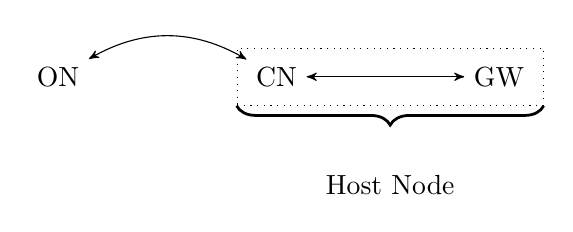
\begin{tikzpicture}[node/.style={circle,draw}]
      \begin{scope}[node distance=2cm]
        \node (a) {ON};
        \node (b) [right=of a] {CN};
        \node (c) [right=of b] {GW};
      \end{scope}

      \begin{scope}[<->,>=stealth',auto]
        \path (a) edge[bend left] (b)
        (b) edge (c);
      \end{scope}

      \node[draw,dotted,fit=(b)(c)](group){};
      \draw[line width=1pt,black,decorate,decoration={amplitude=7pt,brace,mirror}]
      (group.south west) -- (group.south east);
      \node[below=of group,anchor=center]{Host Node};

  \end{tikzpicture}
  \caption{Architecture of a \fitlab node in the testbed}
  \label{fig:fitnode}
\end{figure}

\subsection{The Open Node}

The \ac{ON} is either based on the
\emph{WSN430}\footnote{\url{https://www.iot-lab.info/hardware/wsn430/}}, an
\emph{M3}\footnote{\url{https://www.iot-lab.info/hardware/m3/}} or an
\emph{A8}\footnote{\url{https://www.iot-lab.info/hardware/a8/}} microprocessor,
and a different number of nodes of each type are available depending on the test
site. All nodes except the \emph{A8} node can run \emph{RIOT}
\cite{baccelli2013riot}, \emph{OpenWSN} \cite{watteyne2012openwsn},
\emph{FreeRTOS}\footnote{\url{http://www.freertos.org/}} and \emph{Contiki},
The \emph{A8} only supports
Linux. In addition, the \emph{WSN430}
also has support for \emph{TinyOS} \cite{levis2005tinyos}. Some of the nodes are
mobile and can be configured to move on specified paths through the network.
Their movements can be tracked using \ac{GPS} and are available to the user.

In this evaluation, the \emph{M3} node has been selected for use as the \ac{ON}.
(see \autoref{subsubsec:reasonsm3}).

\subsection{The M3 Node}
\label{subsec:m3}

All experiments in this work have been performed using the \emph{M3} open node.
A simplified block diagram of this node can be seen in
\autoref{fig:m3node}\footnote{\url{https://github.com/iot-lab/iot-lab/wiki/Hardware_M3-node}}.
None of the external peripherals are used in the experiment and can therefore be
disabled to conserve energy.

\begin{figure}
  \centering
  \begin{tikzpicture}
    \node[processor] (cpu)[minimum width=50,minimum height=50] {M3}; %STM32F103RKEY

    \node[memory] (flash) [below of=cpu,below=0.5] {Flash}; %N25Q128A
    \draw[bus,transform canvas={xshift=-10}] (flash) edge node[buslabel] {GPIO} (cpu);
    \draw[bus,transform canvas={xshift=10}] (flash) edge node[buslabel] {SPI} (cpu);

    \node[radio] (wireless) [right of=cpu,above of=cpu,right=0.4] {Radio}; %AT86RF231
    \path[bus] (wireless.240) |- node[buslabel,above] {GPIO} (cpu.10);
    \path[bus] (wireless) |- node[buslabel] {SPI} (cpu);

    \node[system] (usbb) [above of=cpu,above=1] {USB Bridge};
    \path[bus] (usbb) edge node[buslabel] {JTAG} (cpu);
    \path[bus,transform canvas={xshift= 20}] (usbb) edge node[buslabel] {UART} (cpu);

    \node[connector] (oc) [above of=usbb,above=1,minimum width=100] {Open Node Connector};
    \path[bus] (usbb) edge node[buslabel]{USB} (oc) ;
    \path[bus] (oc.190) |- node[buslabel]{GPIO} (cpu.160) ;

    \node[connector] (usb) [right of=oc,below of=oc,right=0.5] {USB};
    \path[bus] (oc) |- (usb);

    \node[processor] (pm) [below of=usb] {Power};

    \node[sensor] (light)   [minimum width=80,below left of=oc,left=1.5] {Light Sensor}; %ISL29020
    \node[sensor] (pressure)[minimum width=80,below of=light] {Pressure Sensor}; %LPS331AP
    \node[sensor] (gyro)    [minimum width=80,below of=pressure] {Gyroscope}; %L3G4200D
    \node[sensor] (magneto) [minimum width=80,below of=gyro] {Magnetometer}; %LSM303DLHC

    \path[bus] (oc.188) |- (light);
    \path[bus] (oc.188) |- (gyro);
    \path[bus] (oc.188) |- (magneto);
    \path[bus] (oc.188) |- (pressure);
    \path[bus] (oc.188) |- node[buslabel,below] {I2C} (cpu.190);
    \path[bus] (gyro)   -| node[buslabel,below] {GPIO} (cpu.120);
    \path[bus] (magneto.10)-| (cpu.120);

    \path[vcc] (pm.210) |- node[below] {+3.3 V} (usbb);
    \path[vcc,orange,text=black] (pm) -- node[auto] {+3.3 V mon.} (wireless);
    \path[vcc] (usb) -- node[left] {+5} (pm);
    \path[vcc] (oc.340) |- node[near start,auto] {+3.3} (pm.165);
    \path[vcc,orange,text=black] (oc.330) |- node[near start,left] {+5} (pm.175);

    \path[vcc,orange,text=black] (pm) |- (1,1.8) -| (cpu.70);
    \path[vcc,orange,text=black] (pm) |- (1,1.8) -- (0.5,1.8);
    \node[rounded rectangle,right of=pm,right=0.1] (gnd) {GND};
    \path[vcc,<->] (pm) -- (gnd);

  \end{tikzpicture}
  \caption{Simplified block diagram of the M3 node}
  \label{fig:m3node}
\end{figure}

% better than wsn430: more diversity, closer to real world deployments in modern iot

\subsubsection{CPU}

The \emph{M3} node features a 32-bit ARM Cortex-M3 based CPU (STM32F103REY)
\cite{stm32f103re} with a maximum clock frequency of 72 MHz. The external clock
runs the \ac{CPU} at this maximum clock frequency, which is to be considered
when evaluating the energy consumption. With all peripherals enabled, this
results in a maximum of 70 mA at 3.3 V \ac{VCC}.

The \ac{CPU} has support for low power modes. When in the \emph{Sleep} mode, the
\emph{CPU} is stopped and all peripherals continue working, in the \emph{Stop}
mode all clocks are stopped and only the contents of \ac{SRAM} and \ac{CPU}
registers are preserved. When in the \emph{Standby} mode the contents of the
registers and \emph{SRAM} are not preserved and the \emph{CPU} can only be woken
up by alarms from the \ac{RTC} or an external reset.

The \ac{JTAG} and \ac{UART} are bridged over \ac{USB} and exposed through the
\emph{Open Node Connector}.

\subsubsection{Flash Memory}

The external \emph{N25Q128} \cite{N25Q128} NOR flash is connected to the
\ac{SPI} of the \ac{CPU} and has a storage capacity of 128 MByte and supports a
maximum frequency of 100 MHz. The \ac{CPU} uses a maxium of 18 MHz for the
\ac{SPI} which results in a maximum 18 Mb/s read / write speed. The
current consumption for page size read / write access is 20 mA.

\subsubsection{Wireless Radio Transceiver}

The \emph{M3} has an ATMEL AT86RF231 2.4 GHz radio \cite{AT86RF231}, which is
connected through \ac{SPI} and \ac{GPIO} and are supplied with 3.3 V. It consumes up to
14 mA when transmitting with a maximum \ac{TX} gain of 3 dBm. For this work, the
\ac{TX} has been set to -7 dBm and the \ac{RX} threshold has been set to -60 dBm
(see \autoref{subsec:rssi}). As such, \ac{TX} needs less than 11 mA when transmitting and
10 mA while receiving. The \emph{6LowPAN} network \cite{rfc4944} stack of \emph{Contiki}
uses the IEEE 802.15.4 support of the transceiver.

\subsubsection{Rationale for Choosing the M3 Node}
\label{subsubsec:reasonsm3}

Instead of the \emph{WSN430}, the \emph{M3} node has been selected for the
evaluation. While the \emph{WSN430} has the advantage of having almost the same processor
(\emph{MSP430}) as the \emph{Z1} node, driver support for the \emph{WSN430}
peripherals like the NOR Flash is based on an an outdated version of
\emph{Contiki}. Moreover, only a very limited amount of nodes of this type had
been available at the time of writing and also not in the linear topology
desirable for the evaluation \autoref{sec:ptopo}.

While the drivers for the \emph{M3} do not support energy estimations using
\emph{Energest} \cite{dunkels2011powertrace}, in-case of the \emph{M3} node,
\emph{Host Node} can record the voltage, current and power consumption of the
\ac{ON} in real time. In doing so, even more accurate and realistic measurements
of the energy consumption are available compared to the profiling done using
\emph{Powertrace}. The \emph{WSN430} for one is not controlled by the \emph{Host
Node} so not all variables that would be desirable for the evaluation, such as
\ac{PCAP} files, can be recorded with it.

Another reason for selecting the \emph{M3} node instead of the \emph{WSN430}
was, that a more powerful processor is available, as will likely be the case in
most modern \ac{IoT} applications, and as such it better models the energy
consumption of these use-cases.

\subsubsection{Considerations for Power Consumption}
One thing to keep in mind when measuring the power consumption at the \ac{ON} is
that only the consumption of the components that can be controlled by the
firmware is monitored. For this, the power management unit monitors the voltage
and current of a separate output besides the one supplying the \ac{USB} bridge. The
power management unit can be supplied both through the open node connector (3.3
V) or directly via \ac{USB} (+5 V).

The core components, on which the experiments in this work have an effect in
terms of power consumption,, are the flash memory, because of the persistence
layer for \ac{RPL}, the \ac{CPU} because the restoring needs some amount of
cycles to complete and the radio, as additional / fewer routing messages may be
sent in the individual modes of the hardened implementation.

The peripheral components, such as the different sensors are not of interest for
the evaluation, since they are not differently depending on whether there are
resets occurring or if the hardened implementation is being used.

\begin{table}
  \centering
  \caption{Consumption estimates for monitored components}
  \begin{tabular}{lr}
    \toprule
    Component & Current Consumption (3.3 V) \\
    \midrule
    CPU & 70 mA \\
    Radio & SLEEP 20 $\mu$A | OFF 0.4 mA | RX 10.3 mA | TX 10 mA\\
    Flash & 20 mA 
  \end{tabular}
  \label{tab:consum}
\end{table}

\autoref{tab:consum} shows the different consumption estimates as they were
obtained from the data sheets of the components. It should be noted, that the
consumption of the \ac{CPU} and the wireless radio could be further reduced by
reducing the clock rate the \ac{CPU} is initialized with and reducing the
transmission power of the radio. Both can be configured using software. For the
evaluation, it was sufficient to keep these values, since a relative comparison
between networks with and without resets should be made.

\subsection{Host Node}

For the \emph{M3} and \emph{A8} nodes, the \ac{HN} serves as both the \ac{GW}
and the \ac{CN}. Each \ac{HN} is directly connected to one or more \ac{ON} using
the \emph{Open Node Connector} and serves the purpose of controlling and
recording the experiment on the \ac{ON}. A simplified block diagram of the
\emph{Host Node} is shown in \autoref{fig:hnblock}.

The \ac{CN} is used for starting and stopping the \ac{ON}, flashing the firmware
and providing a remote \ac{JTAG} debugger via the \ac{USB} bridge on the \ac{ON}
and powering the \ac{ON} from battery or the an external power supply. It also
can monitor the power consumption and record the \ac{RSSI} at the \ac{ON}. As an
alternative to monitoring the \ac{RSSI} the \ac{CN} can record \acp{PCAP} of the
network at the \ac{ON}. For this it has its own radio, similar to the one
supplying the \emph{M3} \ac{ON}. It can also be used for recording sensor data from the
peripherals of the \ac{ON} using \ac{I$^2$C}.

The \ac{GW} part of the \ac{HN} features a more powerful \emph{A8} application
processor and is connected to the site server using a wired
\emph{Ethernet} connection. It is running \emph{Linux} and can provide the
\ac{HN} with network access for applications such as running a remote debugger,
flashing the firmware and starting and stopping the node. It also stores the
measured data from the \ac{CN} which then periodically is fetched by the
site server.

Both the \ac{CT} and the \ac{AM} of the power management unit are configurable
in the profile of the experiment so that a range of different \ac{PM} can be
used for sampling the consumption.

\begin{equation}
  PM = CT \times AM \times 2
\end{equation}

\begin{figure}
  \pgfdeclarelayer{background}
  \pgfdeclarelayer{foreground}
  \pgfsetlayers{background,main,foreground}

  \centering

  \begin{tikzpicture}
    % CN part

    \node[processor] (cpu)[minimum width=50,minimum height=50] {M3};
    \node[radio] (wireless) [right of=cpu,right=0.5] {Radio};
    \node[system] (bridge) [below of=cpu,below=0.5] {USB Bridge};

    \path[bus] (bridge.120) -- node [buslabel,left] {JTAG} (cpu.260);
    \path[bus] (bridge.60) -- node [buslabel,right] {SPI} (cpu.280);

    \path[bus] (wireless.north west) -- node [buslabel,above] {SPI} (cpu.19);
    \path[bus] (wireless.south west) -- node [buslabel,below] {GPIO} (cpu.-19);

    \begin{pgfonlayer}{background}
      \node [draw,fit=(cpu)(wireless)(bridge),label=above:\tiny{Control Node},fill=tubsGray20] (cn) {};
    \end{pgfonlayer}

    \node[processor] (a8) [minimum width=100,minimum height=100,left of=cn,left=4,above of=cpu] (a8) {A8};
    \node[system] (eth) [below of=a8,below=1] {ETH SW};
    \node[connector] (eth0) [below of=eth,right of=eth,below=0.001] {ETH};
    \node[connector] (eth1) [below of=eth,below=0.001] {ETH};
    \node[connector] (eth2) [below of=eth,left of=eth,below=0.001] {ETH};
    \path[bus] (eth) -- node[buslabel,above] {ETH} (a8);
    \path[bus] (eth1) -- (eth);
    \path[bus] (eth0) |- (eth);
    \path[bus] (eth2) |- (eth);

    \node[system] (uhub) [above of=a8,above=2,left of=a8] {USB Hub};
    \path[bus] (uhub) -- node[buslabel,below] {USB} (a8.120);

    \node[connector] (usb0) [above of=uhub] {USB};
    \node[connector] (usb1) [above of=uhub,left of=uhub] {USB};
    \node[connector] (usb2) [above of=uhub,right of=uhub] {USB};
    \path[bus] (usb2) |- (uhub);
    \path[bus] (usb0) -- (uhub);
    \path[bus] (usb1) |- (uhub);

    \node[system] (ubridge2) [right of=uhub,right=2,above of=a8,above=1] {USB Bridge};
    \path[bus] (ubridge2) -- node[buslabel,below] {UART} (a8.60);

    \node[connector] (onc) [minimum width=200,right of=usb2,right=0.5] {Open Node Connector};

    \node[connector] (pwr) [right of=onc,right=3] {Power};

    \node[processor] (pwrmgnt) [below of=pwr,below=1] {Power Mgnt};

    \node[processor] (cmsr) [below of=pwrmgnt,left of=pwrmgnt,left=2] {Current Msr};

    \path[bus] (ubridge2) |- node[buslabel] {USB} (onc.south west);
    \path[bus] (eth.north east) -| node[buslabel] {ETH} (onc.187);
    \path[bus] (bridge.north west) -| node[buslabel] {UART} (onc.190);
    \path[bus] (cpu.160) -| node[buslabel,left] {GPIO} (onc.192);
    \path[bus] (cpu.north west) -| node[buslabel,right] {I2C} (onc.194);

    \path[vcc,<-] (usb2.south east) |- (3.55,4) -- (pwrmgnt.north west);
    \node[label=above left:\tiny{5V}] at (3.55,4) {};
    \path[vcc] (3.55,4) -| (cmsr.100);
    \path[vcc] (pwrmgnt.north west) -- (onc.south east);
    \path[vcc] (pwr) -- node[buslabel,right] {+3.3V to 5V} (pwrmgnt);
    \path[vcc,<->] (cmsr.north east) |- (pwrmgnt);
    \path[vcc] (pwrmgnt) |- node[buslabel] {+48V} (4.5,-2.4) -| (eth0.east);

    \path[vcc,orange] (pwrmgnt.160) |- (onc.east);
    \path[vcc,orange] (pwrmgnt.160) |- node[buslabel,below] {+3.3V} (1,3.5) -- (cmsr.28);

    \node[draw,rounded rectangle] (gnd) at (2.8,2) {GND};
    \path[vcc] (gnd) |- (pwrmgnt);
  \end{tikzpicture}
  \caption{Simplified block diagram of the Host Node}
  \label{fig:hnblock}
\end{figure}

\section{Physical Topology of the Testbed}
\label{sec:ptopo}

When looking at previous studies, the influence of the physical topology of a
network on the routing topology came to attention. This can be used to
affect the routing decisions of \ac{RPL} and reliably create certain \acp{DAG}
in some cases. Nevertheless, with such a large test network of linearly
distributed, we can study the full range of possible outcomes resulting from
\ac{RPL} being applied to it.

For the evaluation, a large network of 44 nodes that are approximately linearly
distributed inside the test lab has been selected. A map of the test network at
\emph{Inria}\footnote{\url{https://www.iot-lab.info/deployment/lille/}} in
France is shown in \autoref{fig:testbed}, where the red nodes are selected for
our experiment, the grey nodes are mounted at the ceiling over a 1.2 $\times$
1.2 m grid at a height of 2.5 m, yellow nodes are attached to vertical poles at
2.4 m, 1.5 m and 0.6 m high and the green square represents the position of the
server cabinet. Additionally, the floor-plan is shown as an outline.

Nodes participating in the experiment are marked as blue circle. Node \emph{157}
has been statically selected as the root of the \ac{DAG}.

\tikzstyle{cnode}=[circle,fill=tubsLightOrange100,text centered,font=\tiny,fill
opacity=0.5,draw opacity=0.5,text opacity=1.0]
\tikzstyle{snode}=[circle,fill=tubsGray20,text centered,font=\tiny,fill
opacity=0.2,draw opacity=0.2,text opacity=1.0]
\tikzstyle{pnode}=[circle split,draw,text centered,fill=tubsLightOrange20,draw opacity=0.1,text opacity=1.0,fill opacity=0.1,font=\tiny]

%TODO latex number vs strings wtf

\newcommand{\fitnode}[3]{%
  \ifthenelse
  {#3 = 47 \OR #3 = 49 \OR #3 = 51 \OR #3 = 53 \OR #3 = 57 \OR #3 = 59 \OR #3 = 83 \OR #3 = 85 \OR #3 = 87 \OR #3 = 89 \OR #3 = 91 \OR #3 = 93 \OR #3 = 95 \OR #3 = 123 \OR #3 = 127 \OR #3 = 131 \OR #3 = 133 \OR #3 = 151 \OR #3 = 153 \OR #3 = 155 \OR #3 = 157 \OR #3 = 159 \OR #3 = 161 \OR #3 = 192 \OR #3 = 194 \OR #3 = 196 \OR #3 = 198 \OR #3 = 200 \OR #3 = 202 \OR #3 = 204 \OR #3 = 218 \OR #3 = 220 \OR #3 = 222 \OR #3 = 224 \OR #3 = 226 \OR #3 = 228 \OR #3 = 230 \OR #3 = 244 \OR #3 = 246 \OR #3 = 248 \OR #3 = 250 \OR #3 = 252 \OR #3 = 254 \OR #3 = 256}%\isin{47}{ \OR #3 = 47 \OR #3 = 49 \OR #3 = 51 \OR #3 = 53 \OR #3 = 57 \OR #3 = 59 \OR #3 = 83 \OR #3 = 85 \OR #3 = 87 \OR #3 = 89 \OR #3 = 91 \OR #3 = 93 \OR #3 = 95 \OR #3 = 123 \OR #3 = 127 \OR #3 = 131 \OR #3 = 133 \OR #3 = 151 \OR #3 = 153 \OR #3 = 155 \OR #3 = 157 \OR #3 = 159 \OR #3 = 161 \OR #3 = 192 \OR #3 = 194 \OR #3 = 196 \OR #3 = 198 \OR #3 = 200 \OR #3 = 202 \OR #3 = 204 \OR #3 = 218 \OR #3 = 220 \OR #3 = 222 \OR #3 = 224 \OR #3 = 226 \OR #3 = 228 \OR #3 = 230 \OR #3 = 244 \OR #3 = 246 \OR #3 = 248 \OR #3 = 250 \OR #3 = 252 \OR #3 = 254 \OR #3 = 256}}
  {\node at (#1,#2) [cnode] {#3};}
  {\node at (#1,#2) [snode] {#3};}
}

\begin{figure}
  \centering

  \usetikzlibrary{shapes}

  \begin{tikzpicture}
    \draw [black!20] (-0.3,13) -- (7.5,13) -- (7.5,4.8) -- (8.7,4.8) -- (8.7,0.8) -- (4.2,0.8) -- (4.2,-0.6) -- (-0.3,-0.6) -- cycle;
    \draw [tubsBlack!20] (8.7,13) -- (13.2,13) -- (13.2,-0.6) -- (8.7,-0.6) -- cycle;
    \fill [tubsLightGreen] (4.7,12.4) rectangle (5.3,12.9);
    \fill [tubsBlack!20] (-0.3,9.2) rectangle (-0.2,11.9);
    \fill [tubsBlack!20] (-0.3,0.2) rectangle (-0.2,2.6);
    \fill [tubsBlack!20] (0,13) rectangle (2.2,13.1);
    \draw [tubsBlack!20] (-0.4,3.95) rectangle (-0.3,4.1);
    \draw [tubsBlack!20] (-0.4,7.95) rectangle (-0.3,8.10);
    \draw [tubsBlack!20] (4.05,3.75) rectangle (4.2,3.9);
    \draw [tubsBlack!20] (4.05,8.05) rectangle (4.2,8.2);
    \draw [tubsBlack!20] (7.40,8.05) rectangle (7.55,8.2);
    \draw [tubsBlack!20] (8.65,3.75) rectangle (8.80,3.9);
    \foreach \x in {0,1,...,4} {
      \foreach \y in {0,1,...,12} {
        \pgfmathparse{int(29+\x*18+(12-\y))}
        \edef\p{\pgfmathresult}
        \fitnode{\x}{\y}{\p}
      }
    }
    \foreach \x in {0,1,...,2} {
      \foreach \y in {1,2,...,12} {
        \pgfmathparse{int(123+\x*14+(12-\y))}
        \edef\p{\pgfmathresult}
        \fitnode{\x+5}{\y}{\p}
      }
    }
    \foreach \y in {1,2,...,7} {
      \pgfmathparse{int(190-\y)}
      \edef\p{\pgfmathresult}
      \fitnode{8}{\y}{\p}
    }
    \foreach \y in {9,10,...,12} {
      \pgfmathparse{int(191-\y)}
      \edef\p{\pgfmathresult}
      \fitnode{8}{\y}{\p}
    }
    \foreach \x in {0,1,...,4} {
      \foreach \y in {0,1,...,12} {
        \pgfmathparse{int(256-(4-\x)*13-\y)}
        \edef\p{\pgfmathresult}
        \fitnode{\x+9}{\y}{\p}
      }
    }
    \foreach \y in {0,2,...,24} {
      \pgfmathparse{int(25-\y)}
      \edef\p{\pgfmathresult}
      \pgfmathparse{int(\p+1)}
      \edef\q{\pgfmathresult}
      \node at (-0.3,\y/2) [pnode] {\p \nodepart{lower} \q};
    }
    \node at (0,13) [pnode] {27 \nodepart{lower} 28};
    \node at (1,13) [pnode] {45 \nodepart{lower} 46};
    \node at (2,13) [pnode] {63 \nodepart{lower} 64};
    \node at (3,13) [pnode] {81 \nodepart{lower} 82};
    \node at (4,13) [pnode] {99 \nodepart{lower} 100};
    \node at (0,-1) [pnode] {42,43 \nodepart{lower} 44};
    \node at (1,-1) [pnode] {60,61 \nodepart{lower} 62};
    \node at (2,-1) [pnode] {78,79 \nodepart{lower} 80};
    \node at (3,-1) [pnode] {96,97 \nodepart{lower} 98};
    \node at (4,-1) [pnode] {114,115 \nodepart{lower} 116};
    \node at (4.3,0.8) [pnode] {\nodepart{lower} 121,122};
    \node at (5,0.8) [pnode] {\nodepart{lower} 135,136};
    \node at (6,0.8) [pnode] {\nodepart{lower} 149,150};
    \node at (7,0.8) [pnode] {\nodepart{lower} 163,164};
    \node at (8,0.8) [pnode] {\nodepart{lower} 190,191};
    \foreach \y in {0,2,4,6,8} {
      \pgfmathparse{int(177-\y)}
      \edef\p{\pgfmathresult}
      \pgfmathparse{int(\p+1)}
      \edef\q{\pgfmathresult}
      \node at (7.5,\y/2+5) [pnode] {\p \nodepart{lower} \q};
    }
    \foreach \y in {12,14} {
      \pgfmathparse{int(179-\y)}
      \edef\p{\pgfmathresult}
      \pgfmathparse{int(\p+1)}
      \edef\q{\pgfmathresult}
      \node at (7.5,\y/2+5) [pnode] {\p \nodepart{lower} \q};
    }
    \node at (4.2,3.9) [pnode] {\nodepart{lower} 119,120};
    \node at (4.2,8.1) [pnode] {117,118};
  \end{tikzpicture}
  \caption{Positions of nodes inside the Lille testbed}
  \label{fig:testbed}
\end{figure}

\subsection{Radio Distances and RSSI}
\label{subsec:rssi}

Another important consideration when selecting the number of nodes has been the
distance between the nodes. When performing preliminary testing on the formation
of the network, it has been observed that the network quickly broke down after a
larger number of nodes had been started. By default, the \ac{RX} threshold and
the \ac{TX} power of each nodes radio transceiver are configured to such values
that all nodes are within radio distance of each other. When the network starts
up, each node attempts to announce its presence to its neighbors using
\ac{ICMPv6} messages. With the selected number of nodes this causes a sufficient
number of collisions for the back-off procedure of \emph{ContikiMAC} to fail and
thus no messages can be transmitted successfully.

For such a problem, multiple resolutions can be thought of including increasing
the distance between the nodes, reducing the number of nodes and reducing
\ac{TX} power and increasing the \ac{RX} threshold. Since the positions
of the nodes are fixed and the area of the test lab is limited, increasing the
distance between the nodes is not an option. Reducing the number of nodes would
decrease the size of the resulting routing topology, which also is not
desirable. In this case, it has been sufficient to follow the recommended
method\footnote{\url{https://github.com/iot-lab/iot-lab/wiki/Limit-nodes-connectivity}}
for controlling node connectivity and to reduce the transmission gain from 0 dBm
to -3 dBm and increase the sense threshold from -101 dBm to -60 dBm.

\subsection{Maintenance Status of Nodes}

The status of all nodes inside the test lab can be viewed using the \ac{API} of
\fitlab. When observing the set of available nodes, a significant amount of
nodes was not available for experimentation and marked as \emph{down}, which
amounted for about half of all nodes.

\section{Accessing to the Testbed}

\fitlab offers programmable interfaces for setting up and controlling
experiments, and obtaining the results. These interfaces are accessible over the
internet using either the \ac{REST}-\ac{API}. Measurement results can be
obtained through \ac{SSH} from a server that is located at the site. The
different interfaces are depicted in \autoref{fig:access}.

\begin{figure}
  \centering
  \usetikzlibrary{fit}
  \begin{tikzpicture}
    \node (U) at (0,0) [shape=circle,draw,fill=tubsLightGreen20] {User};
    \node (A) at (3,0) [fill=tubsLightOrange20,shape=rounded rectangle,draw] {API};
    \node (S) at (6,0) [fill=tubsLightOrange20,shape=rectangle,draw] {Site Server};
    \path (U) edge [arrows=<->,auto,swap] node {REST} (A);
    \path (U) edge [arrows=<->,bend left] node [auto,swap] {SSH} (S);
    \path (A) edge [arrows=<->] (S);
    \node (n1) at (8.5,-1) [fill=tubsLightBlue20,shape=ellipse,draw] {HN};
    \node (n2) at (8.5,0) [fill=tubsLightBlue20,shape=ellipse,draw] {HN};
    \node (n3) at (8.5,1) [fill=tubsLightBlue20,shape=ellipse,draw] {HN};
    \foreach \n in {n1,n2,n3} \path (\n) edge [arrows=<->,auto,swap] (S);
    \path (A) edge [arrows=<->] (S);
    \begin{pgfonlayer}{background}
      \node [label=above:Intranet,fill opacity=0.2,shape=rounded rectangle,fill=tubsLightViolet80,fit=(n1)(n2)(n3)(S)] {};
      \node [label=below left:Internet,fill opacity=0.2,shape=rounded rectangle,fill=tubsLightBlue80,fit=(U)(A)(S)] {};
    \end{pgfonlayer}
  \end{tikzpicture}
  \caption{Accessing the testbed}
  \label{fig:access}
\end{figure}

\subsection{REST API}

The \ac{REST} \ac{API} is provided by an \ac{HTTP} server that and can access
all site servers and as such can send commands to and query all \ac{HN} at
each side. This section describes methods of \ac{API} that have been used in the
experiments.

The \ac{API} for controlling experiments supports the creation and deletion of
experiments. All previous experiments can be queried for a description of their
settings and resources. Also, the state of each experiment can be monitored.
Each configuration of an experiment includes a unique number by which the
experiment will be identified, a list of resources (e.g. firmwares) and nodes.
Each experiment also includes an association of each node with a firmware file
and a profile.

Profiles are managed independently of experiments, although for each experiment a
different profile can be selected. Profiles describe how the \ac{HN} of a node
will be configured during the experiment. These settings include the whether the
node will be powered from battery of from an external power supply, the settings
for the current measurement unit, and the settings for monitoring the radio of
the \ac{CN}.

New firmware files can be uploaded through the \ac{API} and flashed to either a
selection of nodes or all nodes associated with the experiment. This way it is
possible to assign different firmwares for the \ac{DAG} root and all other
nodes.

\subsection{Site Server}

At each site, a central server takes care of coordinating all nodes
participating in an experiment. It is accessed by the \ac{API} for executing the
functions it exposes through the its \ac{REST} interface. Besides through the
\ac{API}, the site server can also be accessed directly using \ac{SSH}. Both the
server and each \ac{HN} are part of the same \emph{Ethernet} network and
communicate using \ac{TCP}/\ac{IP}.

Measurement data is periodically collected from the different \ac{HN} and stored
inside the home directory of the user running the associated experiment. This
data can then be transferred or examined by the user by executing commands on
the server.

\chapter{Measurement Setup}
\label{chap:setup}

This chapter describes the setup used for configuring, and controlling the
experiments inside the lab. Furthermore,it is described how measurement data are
collected, processed and stored. The general software architecture is shown in
\autoref{fig:components}. The components are distributed across several
different platforms.

Measurement data for multiple parameters were collected from the network. The
variables and their data sources are listed in \autoref{tab:params}. The packet
captures can be substituted with outputs on the serial output. For telling the
energy consumption of an implementation, a \ac{PM} of one sample per second is
sufficient.

\begin{table}[h]
  \centering
  \caption{Measured variables at each node}
  \begin{tabular}{ll}
    \toprule
    Variable & Source \\
    \midrule
    Network latency & PCAP, serial output \\
    Delivery ratio & PCAP, serial output \\
    Control overhead & PCAP, serial output \\
    Number of DIO, DAO & PCAP, serial output \\
    DODAG state & serial output \\
    Routing table & serial output \\
    Node reset times & HN event log \\
    RSSI & HN radio receiver \\
    Energy consumption & HN power monitor \\
  \end{tabular}
  \label{tab:params}
\end{table}

When evaluating such a large set of variables from multiple different sources,
the amount of generated data and if enough processing power and storage space is
available has to carefully considered. \autoref{tab:amountdata} shows the
estimated amounts of data generated for each variable. For 50 runs this merely
amounts to 500 MByte of raw data, which can be further compressed using text
compression, since they, especially in the case of the serial log, contain many
repeating strings.

\begin{table}
  \centering
  \caption{Estimated amount of data generated by an experiment with 44 nodes,
    lasting 600 seconds}
  \begin{tabular}{lrr}
    \toprule
    Source & Single (bytes) & Total (KBytes)\\
    \midrule
    Serial output & 300 & 7920 \\
    Event log & 40 & 1056 \\
    Consumption log & 46 & 1214 \\
    RSSI log & 46 & 1214 \\
    \midrule
    Total & & 11404 \\
  \end{tabular}
  \label{tab:amountdata}
\end{table}

\section{Testlab Nodes}

As previously mentioned in \autoref{sec:architecture}, each node inside the
testlab is consists of the \ac{ON} that runs the firmware supplied by the user
and the \ac{HN} that controls and monitors the \ac{ON}. In this section, the
software running on the node and how data is collected from it is further
described.

\subsection{Open Node}

Each \ac{ON} inside the test lab runs a version of the \emph{Contiki} operating
system. The node at the root of the \ac{DAG} is programmed to act as a sink for
the \ac{UDP} traffic that is periodically emitted the other nodes that act as
sources. Each such packet contains a sequence number. The reception of these
packets at the sink and the emission from the source are logged to the serial
output of the node node. This makes it possible to detect whether a packet has
been received when comparing the log of the sink and that of the respective
sender.

Further entries inside the log on the serial output from each node include the
number of emitted \ac{DIO} and \ac{DAO} messages, changes of the routing table and changes
of the preferred parent.

Different versions of the firmware have been produced for the \ac{DAG} root and
all other nodes in the network. The firmware of the root creates a new
\ac{DAG} with the node itself at the root. All other nodes will attempt to join
this \ac{DAG}.

\subsection{Porting the Firmware}

The firmware supplied to the \ac{ON} comes in different versions which each have
different features enabled. The default configuration of \emph{Contiki} 2.7 with
added device support for the \emph{M3} node is provided by \fitlab. The hardened
implementation has been developed based on an older version of \emph{Contiki}, that
also did not include device support for the \emph{M3} node. In preparation for
the evaluation, the hardened implementation has been ported to this newer version
of \emph{Contiki} and some changes and additions had to be made to take into
account changed software interfaces and device specific differences.

Some build options specific to the \emph{Z1} where required for the hardened
implementation to function. These options have been added as necessary.

A missing consistency check has been discovered when restoring the routing state
from flash memory and has then been added that erases the state from the flash
if an inconsistency is discovered.

When testing the hardened implementation, it came to attention that a restart of
the \ac{DAG} root will result in it becoming unable to reconfigure as the
\ac{DAG} root, leading to the network being unusable until the state is purged
from the flash memory of the root node. This is caused by the root node
restoring the previously recorded \ac{DIO} messages from its flash and replaying
them onto the \ac{RPL} module before it configures itself as the root of a
\ac{DAG}. This leads to it joining an existing \ac{DAG} discovered from the
\ac{DIO} messages. This \ac{DAG} is the same \ac{DAG} as was the node previously
the root of. The node joins this \ac{DAG} and selects one of its nodes as a
preferred parent, setting its own rank to a rank larger than its parent. It is
likely that the new parent node previously had selected the former root node as
a parent. In this case, the new parent node of the former root node discovers
that its own parent has a larger rank than In this case, the new parent node of
the former root node discovers that its own parent has a larger rank than
itself. This triggers the former root node to be dropped as the parent at this
node. Thus the tree looses its root and becomes unusable but also unable to
recover, since the root node believes to be already part of a \ac{DAG} and will
not create a new \ac{DAG} with itself as the root node.

\subsection{Host Node}

The \ac{HN} collects the log output from the \ac{ON} and offers it to
connecting clients of a \ac{TCP} network socket. The \ac{HN} also can record
\acp{PCAP} in the direct vicinity of the \ac{ON} and forwards them in a similar
manner to the serial output. Alternatively, the \ac{HN} can record the local
\ac{RSSI}. For each event, including start, stop and reset of the attached
\ac{ON}, a corresponding entry is appended to an event log. The \ac{HN} can also
record accurate values for the power consumption, voltage and current from the
power management unit of the \ac{ON}.

For the purpose of measuring the energy consumption of the node in
reaction to a transient node failure, a high \ac{AM} can be selected since
\ac{RPL} takes some time to react to the change in the network, so the state
will persist for a multiple second. This way it is possible to reduce
the noise component and acquire more accurate data.

The \ac{HN} stores both the consumption data and the \ac{RSSI} in the
\ac{OML}. These log files are stored locally and periodically collected and
stored by the site server.

\section{Site Server}

At each site, a shared server is provided running a multi-user system
(\emph{Linux}). The server periodically queries the events, \ac{RSSI} and
consumption of each \ac{HN} and for each node in the form of log files, stores
them inside the home directory of the user who owns the experiment. The forwarded
serial output of the nodes and the output of the network sniffer are not stored
directly on the shared server because a large amount of data might be generated
this way. Instead, scripts are provided to aggregate the serial output and
stream of network packages into two aggregate streams of messages. These
streams can then be forwarded and stored for later analysis on the local
computer.

\section{Local Computer}

The local computer submits the experiment to the \ac{API}, controls the execution
of the experiment and collects the results from the site server. The data is
stored, processed and later displayed to the user.

\subsection{Orchestration Scripts}

For the purpose of configuring the experiment through the \ac{API}, an
extendable set of scripts has been created. The \texttt{run} script submits the
configuration of the experiment to the \ac{API}, monitors the state of the
experiment, sets up forwardings for the aggregated serial output and packet
captures and loads and calls into hook functions that can be specified per
experiment. The control flow of the script is shown in \autoref{fig:orchest}.

\begin{figure}[h]
  \centering
  \begin{tikzpicture}
    \tikzumlset{fill class=tubsLightBlue20, fill object=tubsLightBlue20, fill component=tubsLightBlue40}
    \begin{umlseqdiag}
      \umlobject[class=script]{run}
      \begin{umlcallself}[op=pre]{run}
      \end{umlcallself}
      \begin{umlcallself}[op=wait running]{run}
      \end{umlcallself}
      \umlobject[class=hook]{during}
      \begin{umlcall}[op=subshell,type=asynchron]{run}{during}
        \umlobject[class=Subshell]{track}
        \begin{umlcall}[op=subshell,type=asynchron]{run}{track}
          \begin{umlcallself}[op=serial aggregator,type=asynchron]{track}
            \begin{umlcallself}[op=sniffer aggregator,type=asynchron]{track}
            \end{umlcallself}
          \end{umlcallself}
        \end{umlcall}
      \end{umlcall}
      \umlobject[class=hook]{post}
      \begin{umlcallself}[op=wait terminated]{run}
      \end{umlcallself}
      \begin{umlcall}{run}{post}
      \end{umlcall}
      \begin{umlcallself}[op=save results]{run}
      \end{umlcallself}
    \end{umlseqdiag}
  \end{tikzpicture}
  \caption{A Sequence diagram of the orchestration scripts}
  \label{fig:orchest}
\end{figure}

First, the script calls the \texttt{pre} hook function from a script file
associated with the experiment, this function can be used for setting up the
environment at the local computer with settings specific to the experiment. Then
the script sends send the configuration of the experiment together with the
associated firmware files to the \ac{REST}-\ac{API} and waits for the experiment
to be started on the test-lab and stores the ID announced by the \ac{API}.

After the \ac{API} has marked the experiment as \texttt{Running}, the script
proceeds by calling into the \texttt{during} function of the experiment. This
function can be used for manipulating the experiment during its executing. In
the case of the experiments run in the evaluation, this function takes care of
resetting a node at a random time during a phase with resets and flashing the different versions of the firmware at the
required time.

After the \texttt{during} function completes, the orchestration script copies
any further results from the side server to the local computer.

\subsection{Aggregation and Storage}

For the storage and analysis of the measurement data, the local computer connects
to the shared server. The aggregated serial output and \acp{PCAP} are
transported to the local computer on one \ac{SSH} connections and each stored
into a separate files. The local computer also collects the log files containing
the events, energy consumption and \ac{RSSI} from the shared server and stores them for
later analysis.

After all data of an experiment has been collected, the contents of the
different files is pre-processed according to the criteria specified for the
evaluation and this data is then stored into a
\emph{SQLite3} database for later analysis. The main reason for pre-processing
the data is to be able to perform the analysis within adequate computation time.

The pre-processed data is then fetched from the database using \ac{SQL}. Numeric
processing of the data is done using \emph{SciPy}
\footnote{\url{https://www.scipy.org/}}, a software library for scientific
computation that is mostly written in the programming language \emph{Python}
but binds to functions written in lower level programming languages that contain
optimized code for certain tasks. The results of the analysis are then displayed
using \emph{Matplotlib}, a \emph{Python} library for displaying structured
data-sets.


\begin{landscape}

\begin{figure}
  \centering

  \begin{tikzpicture}
    \tikzumlset{fill component=tubsLightBlue20, fill port=tubsLightBlue40}

    \begin{umlcomponent}[x=-0.5,y=15,fill=white]{Testlab Node}
    \end{umlcomponent}
    \begin{umlcomponent}[x=3.5,y=15,fill=white]{Testlab Node}
    \end{umlcomponent}
    \begin{umlcomponent}[x=7.5,y=15,fill=white]{Testlab Node}
    \end{umlcomponent}

    \begin{umlcomponent}[x=-1,y=14,fill=white]{Testlab Node}
    \end{umlcomponent}
    \begin{umlcomponent}[x=3,y=14,fill=white]{Testlab Node}
    \end{umlcomponent}
    \begin{umlcomponent}[x=7,y=14,fill=white]{Testlab Node}
    \end{umlcomponent}

    \begin{umlcomponent}[y=1]{Testlab Node}
      \begin{umlcomponent}{Open Node}
        \umlbasiccomponent{UDP Sink / Source}
        \umlbasiccomponent[y=3]{Logger}
        \umlbasiccomponent[y=6]{Powertrace}
      \end{umlcomponent}

      \begin{umlcomponent}[x=6]{Host Node}
        \umlbasiccomponent{Consumption}
        \umlbasiccomponent[y=2.5]{RSSI}
        \umlbasiccomponent[y=5]{Event Log}
        \umlbasiccomponent[y=7.5]{Sniffer}
        \umlbasiccomponent[y=10]{Forwarded Serial}
      \end{umlcomponent}
    \end{umlcomponent}

    \begin{umlcomponent}[y=1,x=14.5]{Shared Server}
      \umlbasiccomponent[y=0]{API}
      \umlbasiccomponent[y=2.5]{Log files}
      \umlbasiccomponent[y=5]{Sniffer Aggregator}
      \umlbasiccomponent[y=7.5]{Serial Aggregator}
    \end{umlcomponent}

    \begin{umlcomponent}[y=1,x=20,fill=tubsLightGreen20]{Local Computer}
      \umlbasiccomponent[y=12]{Orchestration}
      \umlbasiccomponent[y=8]{Database}
      \umlbasiccomponent[y=4]{Analysis}
      \begin{umlcomponent}[y=0]{Presentation}
        \umlactor[scale=0.5]{User}
      \end{umlcomponent}

      \umlassemblyconnector[interface=Parser]{Database-north-port}{Orchestration-south-port}
      \umlassemblyconnector[interface=SQL]{Analysis-north-port}{Database-south-port}
      \umlassemblyconnector[interface=Python]{Presentation-north-port}{Analysis-south-port}

    \end{umlcomponent}

    \umlbasiccomponent[x=14.5,y=14,fill=tubsLightBlue20]{API Server}
    \umlassemblyconnector[interface=REST,with port]{Orchestration-west-port}{API Server}
    \umlassemblyconnector[interface=SSH,with port]{API Server-south-port}{Shared Server-north-port}

    \umlassemblyconnector[interface=SSH,with port]{Orchestration}{Shared Server}
    \umlassemblyconnector[interface=ON Con,with port]{Host Node}{Open Node}
    %\umlHVHassemblyconnector[interface=Configuration,with port]{API}{Host Node}
    \umlHVHassemblyconnector[with port,arm2=+2cm]{Log files}{Consumption}
    \umlassemblyconnector[interface=Log Collection,with port]{Log files}{RSSI}
    \umlHVHassemblyconnector[with port,arm2=+2cm]{Log files}{Event Log}
    \umlassemblyconnector[interface=TCP,with port]{Serial Aggregator}{Forwarded Serial}
    \umlassemblyconnector[interface=TCP,with port]{Sniffer Aggregator}{Sniffer}
  \end{tikzpicture}
  \caption{Software components used in the evaluation}
  \label{fig:components}
\end{figure}

\end{landscape}
\chapter{Evaluation} % English: Evaluation
\label{chap:evaluation}

This chapter summarizes the results of the experiments. At the center of the
evaluation stands the comparison of the energy consumption of the default
\emph{Contiki}-\ac{RPL} and version with added persistance of routing
information. Another important point is how the network topology behaves in the
different configuration and how the network reacts to resetting nodes. For this,
the power consumption of the individual nodes and the complete network, the stability
of the \ac{DAG} and the performance of the network are evaluated.

\section{Firmware Configurations}
\label{sec:confs}

For the firmware, three different modes have been evaluated. The first mode uses
the default \emph{Contiki}-\ac{RPL} (N), the second uses the hardened implementation with
only the storing of persistent state enabled (H) and in the third mode additionally
the sanity of the routing information is checked using \acp{UID} and the clock
values of the neighboring nodes (HS). Each mode is tested for a network where a
reset occurs (R) and for a network where no resets occur. From this result 6
different variants of the experiment which are shown in \autoref{tab:variants}.

\begin{table}[h]
  \centering
  \caption{Experiment configurations}
  \begin{tabular}{r c c c}
    \toprule
    Test run & Hardened & Sanity & Resets \\
    \midrule
    N   &   &   &   \\
    R   &   &   & X \\
    H   & X &   &   \\
    HR  & X &   & X \\
    HS  & X & X &   \\
    HSR & X & X & X \\
    \end{tabular}
  \label{tab:variants}
\end{table}

\section{Influence of Environmental Factors}

When evaluating the data obtained from \fitlab some environmental factors that
have an influence on wireless transmissions have to be taken into account.

\subsection{Radio Interference}

The radio of the \emph{M3} node uses the 2.4 GHz \ac{ISM} bands. One problem
with this is, that this shared spectrum suffers from interference with other
users since it is widely used for other network applications (e.g. \emph{WiFi}).
This means that interference with surrounding devices in the building and with
other experiments in the testbed is legitimate concern. As long as other devices
use some form of \ac{MAC} that is compatible with the one used in IEEE 802.15.4,
this is less of a problem since different senders is able to
coordinate their transmissions to some degree. Because the complete networking
stack the \ac{ON} uses can be user-defined, as is the case with all software
running on the \ac{ON}, this may not always be given.

In the case of previous experiments by Müller et al. \cite{mueller2017}, this
problem was responded to by only running the experiments at night time, where
other senders are less active. In the case of \fitlab, where experiments
may run unsupervised, this is likely not a valid strategy. Another mitigation that
has been performed is to select channel 16 in the 2.4 GHz spectrum in use for
IEEE 802.15.4 and then capturing traffic that can be seen on this channel. Also,
the \ac{API} allows to monitor if other experiments are scheduled during an
experiment and a more appropriate time can be selected instead.

Since we use almost all nodes that are available for experiments and not down
for maintenance, other experiments are effectively prevented from interfering
with ours. Selecting channel 16, in this case, has also proven to be effective in limiting
interference from other networks.

\subsection{Signal Propagation}

As can be seen in \autoref{fig:testbed}, the test network is located on the floor
of a building. This building has multiple floors. The larger part of the
building on the right is separated from the smaller part of the building on the
left in some places by a wall. There are a few pillars between some of the test
nodes. All of them present obstacles for the propagation of the signal. As for the influence
they have on the experiment, it can be noted that the positions of all obstacles
remains constant during and between each experiment. However, the physical topology
(e.g. which nodes are neighboring each other) changes compared to a strictly
linear topology as suggested by the map.

\section{Topology of the RPL Network}

The topology of the network does have a large influence on how much the network
is affected by a resetting node, as was previously shown by Kulau et al. \cite{kulau2017energy}.
For the different runs of the experiment to remain comparable, it is necessary
that under the same conditions the network obtains a similar topology.

\subsection{Ideal Network Topologies}

As previously established, the affect resetting nodes have on the network
depends on the position and role of the node inside the network.

In a tree-like topology as depicted in \autoref{fig:treetop}, nodes have at most
one alternative parent and the entire sub-tree underneath the resetting node
will be affected as they lose their default route to the root node.

For a mesh-like topology, such as in \autoref{fig:meshstar}, the network may be
able to quickly recover after the nodes have selected one of their alternative
parents.

While these topologies serve the purpose of illustrating which factors play into
the behavior of a recovering network, it is not easily possible to recreate such
topologies in a real-wold scenario, since the topology of the network is limited
by the different configurations \fitlab offers.

\begin{figure}
  \centering
  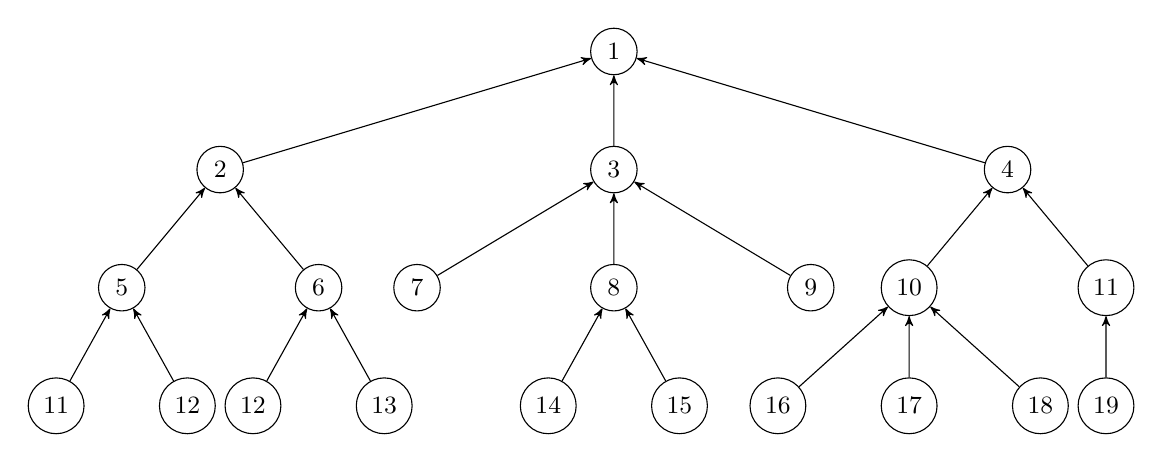
\begin{tikzpicture}[<-,>=stealth', level/.style={sibling distance = 5cm/#1, level distance = 1.5cm}, font = \small, every node/.style={circle,draw}]
    \node {1}
    child { node {2}
      child { node {5}
        child { node {11} }
        child { node {12} }
      }
      child { node {6}
        child { node {12} }
        child { node {13} }
      }
    }
    child { node {3}
      child { node {7}
      }
      child { node {8}
        child { node {14} }
        child { node {15} }
      }
      child { node {9}
      }
    }
    child { node {4}
      child { node {10}
        child { node {16} }
        child { node {17} }
        child { node {18} }
      }
      child { node {11}
        child { node {19} }
      }
    };
  \end{tikzpicture}
  \caption{Tree topology}
  \label{fig:treetop}
\end{figure}

% TODO build in \latex \tikz
\begin{figure}
  \centering
  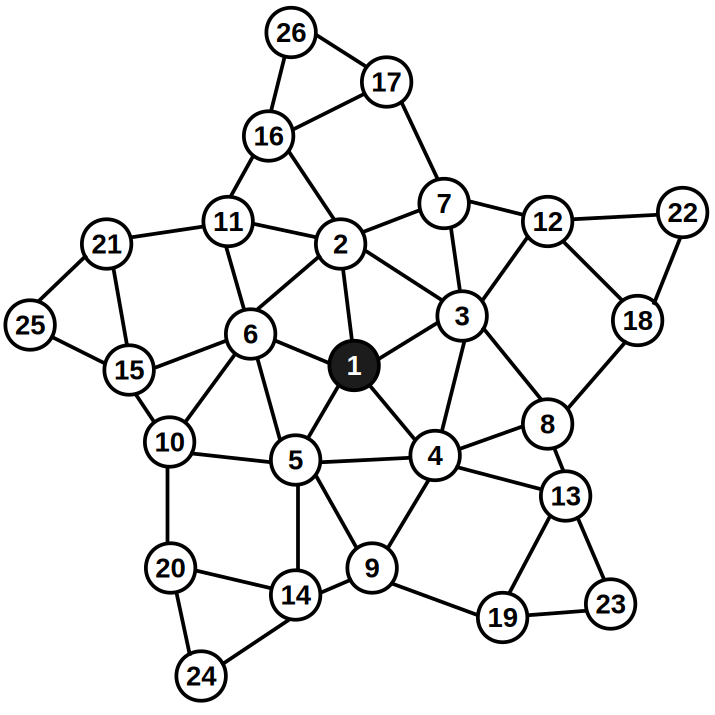
\includegraphics[width=.5\textwidth]{../images/sim_star_new.pdf}
  \caption{Star mesh topology \cite{mueller2017}}
  \label{fig:meshstar}
\end{figure}

\subsection{Measured Topology}

Each topology resulting from any experiments in \fitlab converges upon a very similar
\acs{DAG}. An example of such a \ac{DAG} is shown in \autoref{fig:dagexample}.
One thing that can be observed is that the resulting tree has up to 6 layers.
It should be noted that most nodes are an equal distance to another as displayed
in \autoref{fig:testbed} and the links can be assumed to be of similar quality.

\begin{figure}
  \centering
  \includegraphics[width=\textwidth]{../images/dag.pdf}
  \caption{An example of a DAG generated for the configuration used in the evaluation}
  \label{fig:dagexample}
\end{figure}

\subsubsection{Relationship to the Physical Topology}

One common property of the \ac{DAG}s is that node 159 is the root of the largest
sub-tree. When comparing the nodes of this sub-tree to their positions on the
map, one noticeable property of this sub-tree is that it even contains nodes that
have a closer physical distance to nodes from other sub-trees. In the depicted
tree an example would be node 196 joining the sub-tree of 159 instead of a
acquiring the directly neighboring node 155 as a parent. When comparing to the
shape of the surrounding building these two nodes are divided by two outside
facing walls of the surrounding building, while the path across 159, 200 and 224
is only obstructed by a dry-wall which presents less of an obstacle to the radio
signal.

\subsubsection{Selecting a Node to Reset}

Initial evaluations of the resulting topologies give an indication to which node
needs to reset to have a measureable effect on the network. Node 200 has been
selected to be reset during a single random time during the phases with resets,
R, HR and HSR. The reasons for this are that node 200 has a large enough sub-tree in
most runs of the experiment to affect enough nodes and because it is the node
that is most frequently selected as a preferred parent when connecting the two
halves of the building.

\subsection{Route Stability}

The stability of the network is determined by how stable the conditions are on
which the routing protocol bases its decisions. For a network where resets
occur, these conditions will change upon the reset of a node and the routing
protocol reacts to this situation. Therefore, the number of changes of the
routing decisions is a measure of the stability of the network created by the
routing protocol.

\begin{figure}
  \centering
  \includegraphics[height=.3\textheight]{../images/stability.pdf}
  \caption{Number of changes of the default route of any node during a phase}
  \label{fig:stability}
\end{figure}

\autoref{fig:stability} shows the number of changes of the default route of any
node during each phase of an experiment. The default implementation in phase N
causes the fewest changes if no single node resets occur. The hardened
implementations of H and HS on the other hand lead to more changes. This may be
due to the processing, or restoring and invalidating a previous invalid state from
persistent memory.

The number of changes for the hardened implementations during a phase with
single node resets is smaller than for the default implementation. This means
that the hardened implementations recover more easily from single node resets
than the default implementation does.

\subsubsection{Relation to Location}

\autoref{fig:hmroutes} shows a heat-map of the distribution of default routes
during each phase. Each cell results from the number of times the route has been
selected at the end of an interval of 10 seconds during the phase of an
experiment. This number was then then normalized by the length of the phase
during the experiment, since the length of a phase may vary due to variations in
how fast the test-lab reacts to instructions given by the orchestration
component. Thus, routes that are more often selected are shown in a darker hue,
while routes that are rarely selected are shown in a lighter hue. 

\begin{figure}
  \centering
  \includegraphics[width=\textwidth]{../images/routes.pdf}
  \caption{Heat-map of the normalized choice of default routes for the different
    phases}
  \label{fig:hmroutes}
\end{figure}

The most noticeable thing about the these maps is that the distribution of
routes of routes between the different phases does not vary much, in that the
maps are almost identical. One thing to conclude from this is that the choice
of the \ac{DAG} is not altered in a relevant way by adding the persistance mode
in phase H or additionally validating \acp{UID} in phase HS. This means that
that there is not enabling the hardened implementation in regard to the choice of
an optimal \ac{DAG}.

Another thing to be noted is that the when viewing each row of the map, some
nodes show a distribution of routes which is very dense for a small number of
different neighbors while others do not have such routes. When compared to the
topology of the \ac{DAG}, the nodes that offer more stable routes are generally
inside nodes of the tree (e.g. not leaves). Nodes that tend to change
routes more join the tree as nodes.

The comparison of the phases have resets with their counterparts yields that there
are more changes between the N and the R phase than are between the H and the HR
and the HS and the HSR phases. From this it can be interpreted that more route
changes may have occurred during the reset of the node in phase R. This would
mean that the network is in a more unstable state during R than in HR and HSR.

%\subsubsection{Relation to Rank and Number of Neighbors}
%
%\autoref{fig:rankvsneighvschanges} shows the pairwise relationship of the rank
%of a node, its number of neighbors and the number of changes of its preferred
%parent selection.
%
%% TODO create new figure
%
%%\begin{figure}
%%  \centering
%%  \includegraphics[width=\textwidth]{../images/changes.pdf}
%%  \caption{Rank, default parent changes, number of neighbors}
%%  \label{fig:rankvsneighvschanges}
%%\end{figure}
%
%With increased rank, the number of changes of the preferred parent increases.
%This may cause an increase in energy consumption. One possible explanation may
%be that the possible number of nodes that may fail along the path to the sink is
%increased when a node has a higher rank. This is supported by the fact that the
%increase in changes is higher for the phases that include resetting a node. As
%such it can be expected to see a noticeable increase in power consumption for
%these phases (see \autoref{fig:consum-rank.pdf}).

\subsection{Convergence Time}

When considering the resulting routing topology, the time it takes the network
to converge upon one topology is also of interest. A larger amount of
routing messages will have to be transmitted, the longer some single node in the
network takes to acquire a preferred parent.

\autoref{fig:convtime} shows the convergence time of the network for each phase.
The phases without resets are grouped to the left and on the right are displayed
the phases with resets.

\begin{figure}
  \centering
  \includegraphics[height=0.3\textheight]{../images/convergence.pdf}
  \caption{Network convergence time for each phase}
  \label{fig:convtime}
\end{figure}

It is noticeable that both the H and HS phases, which use the hardened
implementation, have generally longer convergence times than the default
implementation of \ac{RPL}. In the case of the restoration of the routing state
from persistent memory, as in phase R and HS, all previously recorded \ac{DIO}
messages will be replayed to the \ac{RPL} module of \emph{Contiki}. This implies
that the time it takes to process these messages and make changes to the saved
\ac{DAG} and routing table adds to the time it takes to choose a preferred
parent and therefore lengthens the network formation time. It can be assumed
that much of this time is spend writing and reading this data from the peristant
memory.

In the case of the HS and HSR phases, additional \ac{DIO} messages are
exchanged to verify the stored routing information and messages before restoring
them. These messages contain \acp{UID} to identify the information and measure
the freshness of the information using the clock the implementation keeps for
the local routing information. Presumably, the time it takes to exchange these
messages further adds to the delay until a suitable preferred parent is selected
for each node.

Another thing that is remarkable is how much the convergence time varies for the
H and HS phases compared to the phases without the hardened implementation,
regardless of whether there are resets or not. As a consequence, the network
forms in a more reliable manner in the default implementation.

An interesting observation about the difference in the convergence time between the
phases with resets and those without is that generally the convergence time is
shorter for a network with resets. It would be expected that the inverse of this relation would
be the case. The exact reason for this can only be speculated upon. If a reset
occurs during the initial formation of the \ac{DAG} during a phase, the
resetting node might not partake in the formation of the network. This then
would mean that less alternative paths inside the network exist from which to
choose which might lead to the network converging faster.

% TODO network convergence time derectly after reset


\section{Energy Consumption}

% TODO error from measuring 2nd phases --> indirect comparison by # messages ...
This section discusses the energy consumption of the test
network and how it changes based on the implementation in use and whether a single
node reset occurs. \autoref{fig:consphases} shows the total energy consumption
of the network during the different phases. Nodes 200 and 157 have been excluded
since they act as the resetting node and the root node.

\begin{figure}
  \centering
  \includegraphics[height=0.3\textheight]{../images/consumption-phases.pdf}
  \caption{Total consumption except nodes 200 and 157}
  \label{fig:consphases}
\end{figure}

For a network in which no resets occur, the consumption of the default
implementation (N) is significantly lower than for both versions of the hardened
implementation (H, HS). One possible factor in this may be the energy spend on writing
the persistent state to the flash memory. Another may be the additional
computing time spend on processing the restored state and in case of the HS
phase, the exchange of \ac{DIO} messages.

This effect is amortized when recovering from a reset in the phases HR and HSR,
where the default implementation uses more energy than the hardened version (HR).
For instances, the extended hardened implementation (HSR) uses less power than
the default implementation, but the mean of the consumption is higher for HSR.
This means that the additional exchange of messages to verify the state stored
in persistent memory consumes more energy on average than the restoring of the
persistent state saves.

\subsubsection{Constant error between consecutive phases}

The comparison of the phases in which no resets occur (N, H, HS) versus the
phases with resets (R, HR, HSR) yields, that a smaller energy consumption is
measured for the phases with resets. 

For each firmware, the phase with and without resets run consecutively. For each
series of measurements for each individual node the power consumption of each
second phase is smaller over the complete duration of the phase. This leads to
the conclusion that this behavior is not triggered by the single node reset,
but rather caused by an external factor.

For this reason, the measured values of the energy consumption of the
individual phases are only valid for comparison between phases that either have
resets or do not. For the comparison of the phases that use the same firmware
(e.g. N and R) other variables can be used, such as the number of protocol
messages and the number of changes of the preferred parent.

%TODO measurement sequence

\subsection{Consumption of the DAG Root and Resetting Node}

\autoref{fig:cmpsinkreset} shows the total consumption of the network, except for
the sink node and the resetting node. Node 123 is shown for comparison as it is
close to the average of the consumption of all other nodes.

\begin{figure}
  \centering
  \includegraphics[height=0.3\textheight]{../images/consumption-hosts.pdf}
  \caption{Energy consumption for the sink node and the resetting node}
  \label{fig:cmpsinkreset}
\end{figure}

When viewed separatly, the energy consumption of these nodes varies widely from
the other nodes and from each other as seen in \autoref{fig:cmpsinkreset}. In
the case of the sink node, this is because, to minimize packet loss, its radio
is forced to the \ac{RX} state and it acts as the \ac{UDP}-sink and thus has to
process many packets. The resetting node can be expected to consume much less
power while it is resetting, since a restart involves power-cycling the node.
Thus, for the phases with resets (R, HR, HSR), the consumption is lower for node
200 and 157 consumes significantly more energy than the average node. Such a
node would typically be powered from the power grid.

%\subsection{Relation to Rank}
%
%% TODO
%
%As can be viewed from \autoref{fig:relconsum}, the energy consumption increases
%with the rank for HS and HSR. For the N and H, this relationship is inverted.
%
%\begin{figure}
%  \centering
%  \includegraphics[height=0.4\textheight]{../images/consumption-regress.pdf}
%  \caption{Relation of rank and consumption of a node}
%  \label{fig:relconsum}
%\end{figure}

\subsection{Relation to Position inside the Testbed}

\autoref{fig:posenergy} displays the positions of the nodes inside the testbed.
Every cell shows a color representing the relative energy consumption associated with
that node. Lighter colors represent a lower energy consumption, whereas darker
colors represent a higher energy consumption.

\begin{figure}
  \centering
  \includegraphics[width=0.4\textheight]{../images/consumption-nodes.pdf}
  \caption{Energy consumption of nodes arranged by their position}
  \label{fig:posenergy}
\end{figure}

One noticeable thing about this distribution is that node 87 has the highest
energy consumption in all phases. When looking at the \ac{DAG}, this node is
mostly located at a lower rank. Nodes that are physically located closer to the
root node 157, tend to have a lower energy consumption than surrounding nodes.
A wall separates the nodes 192, 194 and 196 from 157. This coincides with these
nodes having a higher energy consumption.

\section{Network Performance}

In this section, the network performance and the control overhead for the
different phases is evaluated.

\subsection{End-to-End}

\autoref{fig:perf} shows the average end-to-end delay for all nodes during each
phase of the experiment. While in phase H, shorter delays are possible. At the
same time, the distribution varies more. With the added sanity checks in phase
HS, the distribution is more focused around 2 ms. The default implementation in
N lies somewhere in-between the two.

%\begin{figure}
%  \centering
%  \subfloat[delay]{{\includegraphics[width=.5\textwidth]{../images/performance-delay.pdf}}}%
%  \qquad
%  \subfloat[jitter]{{\includegraphics[width=0.5\textwidth]{../images/performance-jitter.pdf}}}%
%  \subfloat[loss]{{\includegraphics[width=0.5\textwidth]{../images/performance-loss.pdf}}}%
%  \caption{Delay, jitter, loss for each phase}
%  \label{fig:perf}
%\end{figure}
\begin{figure}
  \centering
  \subfloat[delay]{{\includegraphics[width=.5\textwidth]{../images/performance-delay.pdf}}}%
  \subfloat[loss]{{\includegraphics[width=.5\textwidth]{../images/performance-loss.pdf}}}%
  \caption{End-to-end delay and package reception rate}
  \label{fig:perf}
\end{figure}

The packet loss during each phase is displayed in \autoref{fig:perf}. For a
scenario without single node resets, the default implementation fares best,
while in a scenario with single node resets the hardened version without the use
of \acp{UID} looses the fewest packets. If additionally the sanity checking
of the persistent state is enabled, the most packets are lost.

One possible explanation for this is that if the persistent state is directly
restored, most of the time this state is sufficient for the forwarding of newly
arriving packets. If the node must first validate the saved state, it looses
time during which arriving packets may be dropped. This would suggest that the
validation of the saved state is actually slower than the default method of
recovery.

\subsection{Control Overhead}

The number of messages that need to be emitted during the repair operations of
the \ac{DAG} determines the utilisation of the radio of the node. It is to be
expected that a large part of the energy consumption of the each node is
determined by the number of messages it emits. Thus, when evaluating the
efficiency of the different implementations and the impact of the single node
resets, the overhead of messages that are transmitted by the implementation
serves an important measure.

\autoref{fig:overhead} shows the overhead created by control messages that were created
during each phase by message type. For each type, the default implementation
creates the fewest additional messages of any type, while the number of messages
is the highest for the implementation used in HS. This may be attributable to
the higher number of messages exchanged during the validation process. The
larger number of overhead created during phase H is likely due to an old state
being restored from previous runs and then invalidated.

\begin{figure}
  \centering
  \includegraphics[height=0.3\textheight]{../images/performance-overhead.pdf}
  \caption{Overhead created by \ac{RPL} messages}
  \label{fig:overhead}
\end{figure}

For the phase R the overhead is higher than for the phase N, where no resets
occur. At the same time the inverse is true for the phases with hardened
implementations. Here the effect of an old state being restored and then
invalidated is later canceled out, when restoring the state after the node reset
occurred and actually less overhead is created than for the default implementation.

It should also be noted that there is no significant difference for the overhead
during the HR and HSR phases, which means that the implementation used in HS and
HSR does not offer a clear benefit over the implementation used in H and HR in
terms of message overhead.

\subsubsection{Consumption}

\begin{figure}
  \centering
  \includegraphics[width=\textwidth]{../images/performance-consumption.pdf}
  \caption{Relationship between overhead and energy consumption}
  \label{fig:overconsum}
\end{figure}

As can be seen from \autoref{fig:overconsum}, the number of control messages
correlate to the observed consumption. For a larger overhead, the total
consumption increases proportionally.

\acresetall
\chapter{Conclusion}

% - evaluate effect of transient node resets + hardened implementation
% - create tools for setting up + measuring + analysing experiments
% - \fitlab 
% - stable topology
%   --> comparable
% - transient node resets are a thing
%   - if reset: changes ++
%   - less with hardening
%    - if no reset: less good --> depends on use-case
% - convergence time
%    - restoring state takes time
%    - restoring wrong state even more --> validation helps
% - performance: delay, packet loss
%   - hardened implementation loses fewer packets when used without restore UID
%   - but both worse without single node reset

The topic of this work has been to evaluate the reset of single node restarts
and the possibly resulting transient node failures on a \ac{WSN} which uses
the \ac{RPL}. The evaluation has been performed using \fitlab. For this software has
been created to automate the experiments using the existing infrastructure
provided by \fitlab and analyze the data obtained from the experiments. For
running the hardened implementation in \fitlab, the implementation has been
ported to a newer version of \emph{Contiki} that has device support for the
sensor nodes.

Each experiment has been performed in six different phases, where the first two
(N and R) use the default implementation of \ac{RPL} in \emph{Contiki}, the
second pair (H and HR) uses the hardened implementation \cite{mueller2017} and
the third pair (HS and HSR) uses the hardened implementation that also checks
the validity of the restored routing information.

First, the \ac{DAG} that results from each experiment has been compared and
checked for variances. It has been discovered that, using \fitlab it is possible
to reliably create a tree where a certain node (e.g. the node to be
reset during R, HR and HSR) joins the \ac{DAG} at a certain rank. This means
that comparable results can be obtained for the effect of single node resets.

Next, the instability of the \ac{DAG} has been evaluated by counting the number
of changes that occur during each phase. It has been observed that a single reset
will trigger a large amount of changes in the \ac{DAG}, which will result in a
higher energy consumption. If such resets occur, both versions of the hardened
implementations will reduce the  number of changes to the
\ac{DAG}, but will increase the number of changes if no resets occur, in which
case the default implementation performs better.

From observing the network convergence times for \ac{RPL} for each
implementation with and without single node resets, it can be concluded that
restoring the state takes time, during which arriving packets will be lost. The
hardened implementation, but without the validity checks enabled, performs best in
reducing the time packets are dropped while the node recovers from its reset. It
has been discovered that the validity checks that involve the exchange of
\ac{DIO} messages take longer than recreating the state without restoring it
from persistent memory.

The final part of the evaluation looked at the message overhead generated by
each implementation and for a network with and without single node resets. Here
it has been observed, that the default implementation creates the lowest
overhead for a scenario without single node resets, while the hardened
implementations create a large overhead if no single node reset occurs. For a
scenario where single node resets occur, both of the hardened implementations
manage to achieve a smaller message overhead than the default implementation.

In general, it can be concluded that the energy consumption of the hardened
implementation is significantly higher than for the default implementation if no
single node resets occur. If single node resets occur, the hardened
implementation will only have a small advantage over the default implementation
in terms of energy consumption.

\bibliographystyle{abbrv}
\bibliography{../bibliography}

\appendix

\chapter{Contents of the CD}

\begin{description}[style=nextline]
    \item [data.tar.xz] xz compressed tar archive of the complete data for each experiment
    \item [contiki-inga.bundle]  GIT bundle of the \emph{Contiki} source code used in the evaluation
    \item [2017-schubert-fitiot.bundle]  GIT bundle of this thesis and all scripts for the evaluation
\end{description}

\end{document}
